\cleardoublepage

\chapter{Optimización de la eficiencia energética de OmpSs sobre arquitecturas asimétricas}
\label{ch:chapter5}

\section{Descripción de la estrategia de optimización}

\todo{Descripción general, similar a la del capítulo anterior. Un resumen, sin más.}

\subsection{DVFS sobre la arquitectura big.LITTLE}
\label{sec:DVFS_BIGLITTLE}

\todo{Hablar de DVFS, frecuencias soportadas por cada SoC, libcpufreq\ldots}

\subsection{Evaluación de rendimiento/eficiencia energética de las tareas}

\todo{Pequeña descripción de rendimiento/eficiencia basada en los resultados que se muestran,
para motivar el trabajo.}

\begin{figure}
  \centering
    \begin{subfigure}{0.45\textwidth}
      \centering

      \begin{framed}
        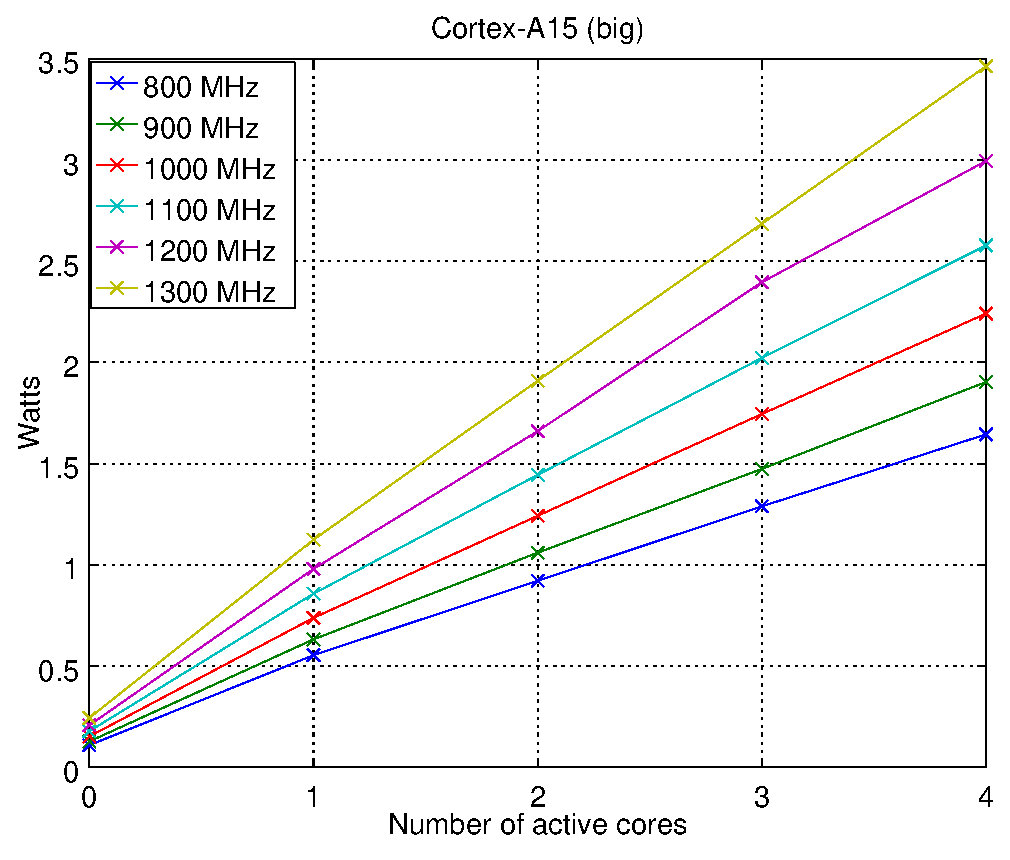
\includegraphics[width=1\linewidth]{Plots/Modelos_consumo/odroid_big.eps}
        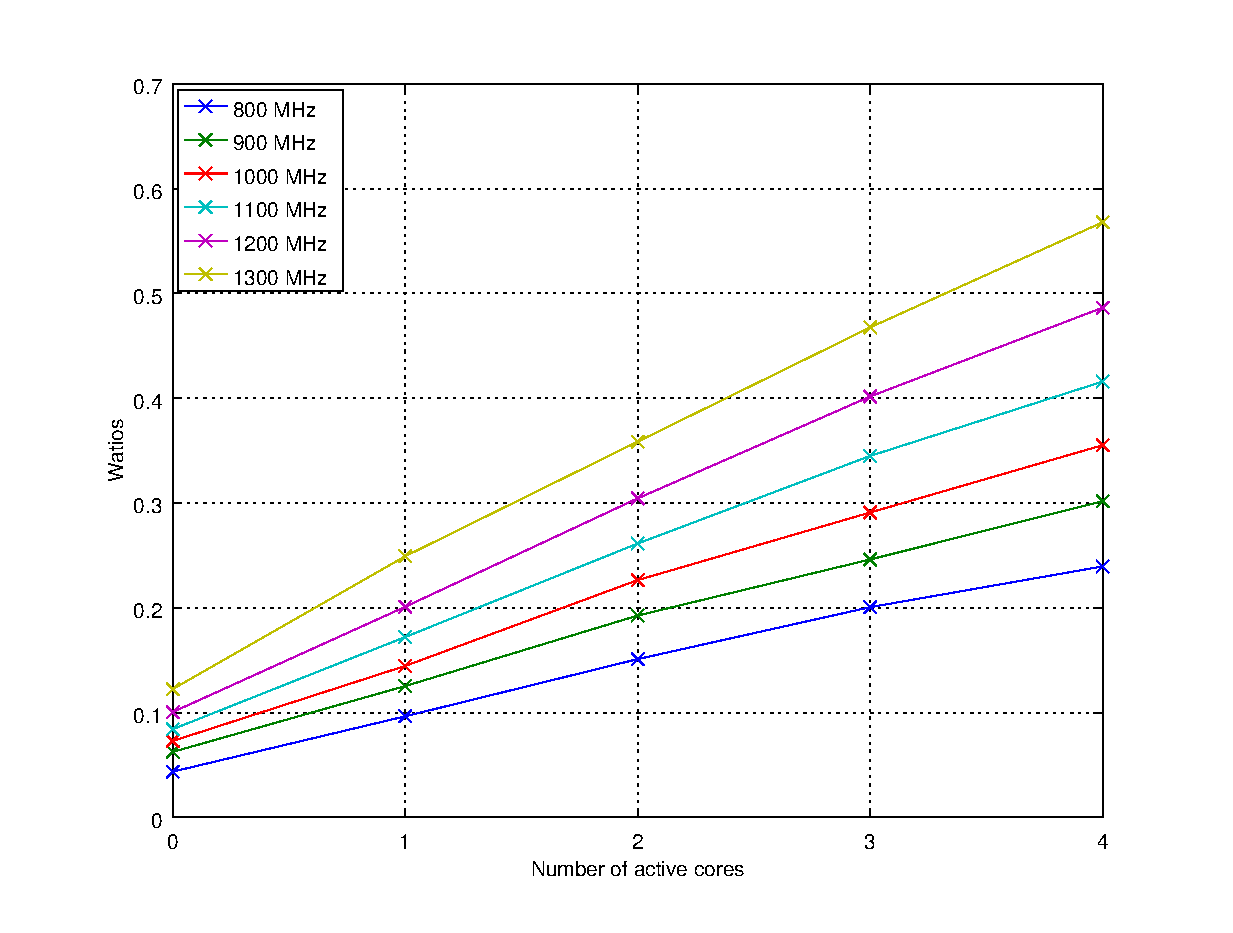
\includegraphics[width=1\linewidth]{Plots/Modelos_consumo/odroid_little.eps}
      \end{framed}
      \caption{\odroid}
      \label{fig:modelo_consumo-odroid}

    \end{subfigure}
%
    \begin{subfigure}{0.45\textwidth}
      \centering
      \begin{framed}
        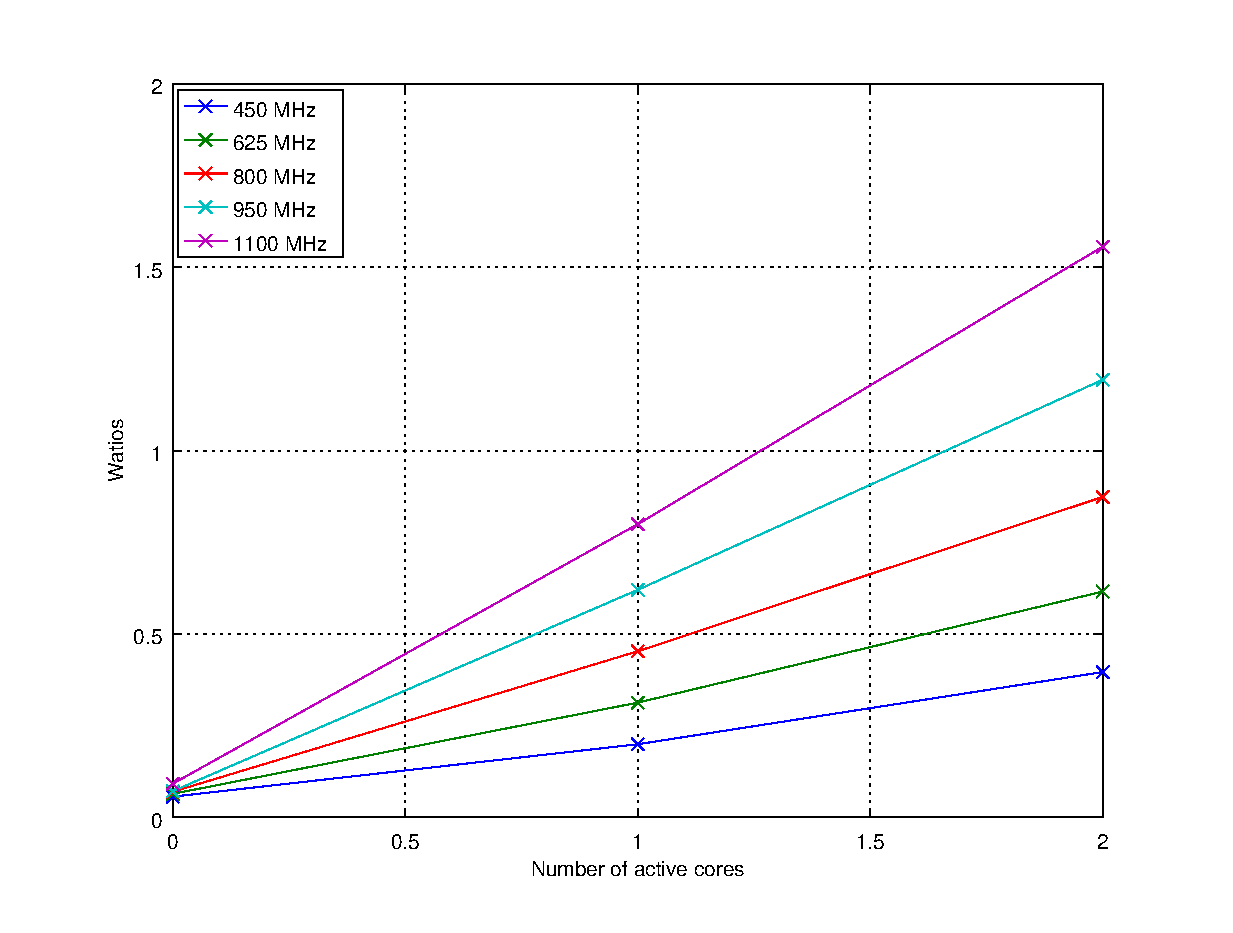
\includegraphics[width=1\linewidth]{Plots/Modelos_consumo/juno_big.eps}
        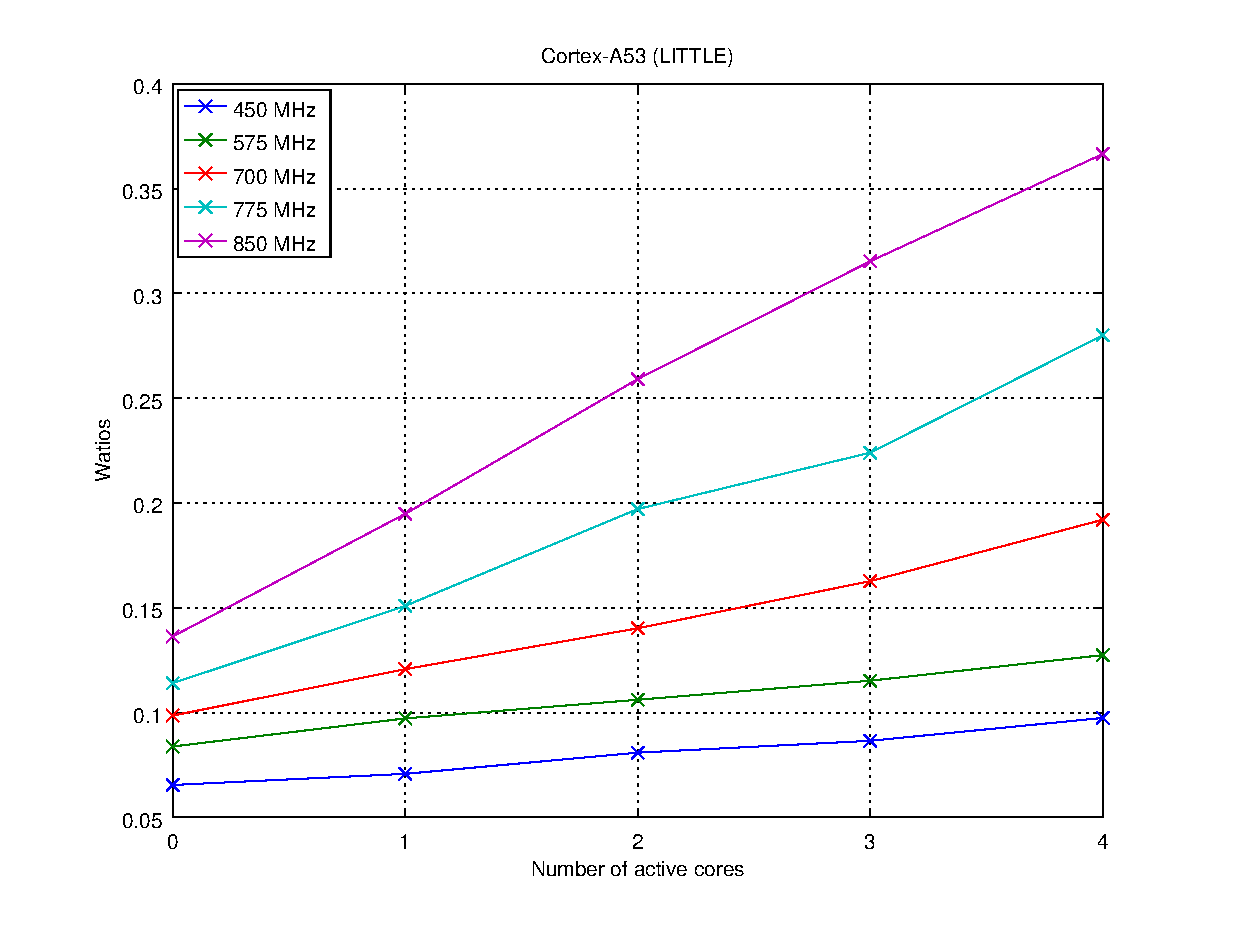
\includegraphics[width=1\linewidth]{Plots/Modelos_consumo/juno_little.eps}
      \end{framed}
      \caption{\juno}
      \label{fig:modelo_consumo-juno}
    \end{subfigure}  

	\caption{Medidas de consumo energético por núcleo y plataforma. \todo{Hay algunas etiquetas en inglés (eje X) y otras en castellano (eje Y)}}
  \label{fig:modelo_consumo}
\end{figure}





\section{Políticas de reducción de consumo}
En esta sección se detallan las diversas políticas desarrolladas para 
reducir el consumo energético en una arquitectura asimétrica. Las políticas
se encuentran divididas en dos grandes grupos: un primer grupo formado por
politicas basadas en {\em escalado de frecuencia}, y un segundo grupo formado por
políticas encargadas de modificar la {\em asignación de las tareas} a los
diferentes \wts generados por el \emph{runtime} (y por tanto, a los diferentes núcleos que
componen la arquitectura).

\subsection[{Políticas basadas en escalado de frecuencia (P1, P2, P2' y P3)}]{Políticas basadas en escalado de frecuencia}


\subsubsection{Política P1}

Durante la ejecución de un programa paralelo mediante un paradigma basado
en tareas, es común que, en cierto punto de la ejecución paralela,
la mayor parte de tareas listas para ser ejecutadas
sean tareas pertenecientes al {\em camino crítico}, provocando que nuevas tareas no puedan 
pasar a considerarte listas para ejecución hasta que las tareas críticas finalicen. 

Este comportamiento puede observarse en una aplicación cuyo grafo de
dependencias se encogiera muy rápidamente en algún punto intermedio de la
ejecución, para luego volverse a expandir rápidamente (un árbol con forma
de diábolo). En este tipo de árbol, las tareas ``centrales''
serían críticas, ya que son prioritarias para que la ejecución paralela
prosiga, y además, en el momento que esto ocurra, un gran
número de tareas serán liberadas para ser ejecutadas y
poder continuar la ejecución del problema.

Este problema, aplicado al planificador \botlev, (descrito en la
sección~\ref{s3:botlev}) supondría que en el momento en el que el árbol se
estreche, la cola de tareas no críticas tendría un tamaño muy inferior a la
de tareas críticas, y por tanto los cores \LITTLE tendrían mucha menor carga
de trabajo que los cores \BIG. Este fenómeno se da mientras los cores big
finalizan la ejecución de sus tareas críticas y se liberan más tareas para
ejecutar en los cores \LITTLE.

Una forma de intentar paliar este problema consiste en forzar a que los
núcleos lentos también ejecuten tareas críticas; este decisión, sin embargo, puede provocar 
un retraso en la finalización de las tareas críticas, ya que aunque su ejecución
puede comenzar antes (pues se disponen de más núcleos para distribuir
el mismo número de tareas), el rendimiento de los núcleos \LITTLE es muy
inferior que el de los cores \BIG, provocando retrasos en la ejecución e
incluso llegando a agravar el cuello de botella anteriormente mencionado.

La política P1 intenta solventar este problema desde un enfoque distinto. La
idea principal consiste en aprovechar los períodos de tiempo en los que la carga 
de trabajo sobre los núcleos lentos es menor para disminuir el consumo energético, 
{\em forzando una reducción de frecuencia} sobre el cluster \LITTLE. 
Como se podía ver en la Figura~\ref{fig:modelo_consumo}, reducir la frecuencia al cluster \LITTLE
implica que la potencia instantánea disipada disminuye. Aunque es cierto que al
reducir la frecuencia de los núcleos el tiempo empleado en ejecutar una tarea
aumenta, esta técnica únicamente se aplica en aquellas fases de la ejecución paralela en las que
la ejecución está limitada por el gran número de tareas críticas y el
bajo número de tareas no críticas; por tanto, es esperable que el impacto final en el
rendimiento no sea elevado, y sí lo sea la reducción de consumo energético.

La forma en la que se ha aplicado esta política sobre \botlev
consiste en monitorizar constantemente el número de tareas, tanto críticas
como no críticas, listas para ser ejecutadas (reflejado en el tamaño de las
colas internas del planificador), y actuar en función a la relación entre
el tamaño de ambas colas. La Figura~\ref{s5:fig:listing-p1} muestra un
fragmento esquemático del código encargado de realizar esta tarea. El
método es invocado cada vez que el tamaño de una cola es modificado (ya sea porque
una tarea comienza su ejecución, o porque una tarea se encuentra lista para
ser ejecutada y es insertada en una cola). Como se puede observar en la
línea~\ref{s5:lst:p1-calculoPrincipal(a)}, la frecuencia a la que cambiar
el cluster se calcula como una proporción directa entre el tamaño de ambas
colas; así, por ejemplo, si el número de tareas críticas es el doble que el de las
tareas no críticas, la frecuencia se disminuye un ``escalón''; si el tamaño
es el triple, la frecuencia se disminuye hasta el tercer escalón de
frecuencia, etc. Cabe recordar que los valores de frecuencia que puede tomar el
cluster están limitados por el kernel del sistema operativo, como se
mencionó en la sección~\ref{sec:BIG_LITTLE}. La
línea~\ref{s5:lst:p1-calculoPrincipal(b)} asegura que la frecuencia final
no es menor que la menor frecuencia soportada. Por tanto, en esta política,
el cambio de frecuencia en el cluster se realiza de manera
escalonada según varía el tamaño de las colas.

\begin{figure}
  \centering

  \begin{lstlisting}[language=C++]
int P1(int bigQueueSize, int littleQueueSize){
  int nxtFreq;
      
  if( littleQueueSize==0 ) nxtFreq = FreqCfg::minLittleFreq; |\label{s5:lst:p1-casoEsp1}|
  else if( bigQueueSize==0 ) nxtFreq = FreqCfg::maxLittleFreq; |\label{s5:lst:p1-casoEsp2}|
  else{
    int idx = min((bigQueueSize / littleQueueSize), |\label{s5:lst:p1-calculoPrincipal(a)}|
                   FreqCfg::maxIdxLittle );         |\label{s5:lst:p1-calculoPrincipal(b)}|
    nxtFreq = FreqCfg::littleFreqs[idx];
  }
  return changeLittleFreq(nxtFreq);
}
\end{lstlisting}

  \caption[Fragmento de código esquemático para la política P1]
  {Fragmento de código esquemático para la política P1.}
  \label{s5:fig:listing-p1}
\end{figure}

Adicionalmente al comportamiento general de esta política, hay que
distinguir dos casos especiales que merecen ser mencionados: el caso en el
que no exista ninguna tarea crítica lista para ser ejecutada, y el caso
opuesto, en el que todas las tareas listas sean críticas y los cores lentos
estén totalmente ociosos. En estos casos, las
líneas~\ref{s5:lst:p1-casoEsp1}-\ref{s5:lst:p1-casoEsp2} se encargan de
aumentar la frecuencia al máximo directamente en caso de que todas las
tareas sean no críticas, o de disminuir la frecuencia al mínimo en caso de
que no exista ninguna tarea no crítica que ejecutar.

La Figura~\ref{s5:fig:P1-evo} muestra el comportamiento de esta política
para una factorización de Cholesky sobre una matriz de dimensión
$1024 \times 1024$ usando precisión simple y dividida en bloques de
$64 \times 64$ elementos. La gráfica superior muestra el estado de las
colas durante la ejecución del problema, mientras que la gráfica inferior
muestra la frecuencia del cluster de núcleos \LITTLE en cada momento de la
ejecución del problema. Como se puede apreciar, al inicio de la ejecución
(cuando el número de tareas críticas es elevado), la frecuencia se reduce
de manera escalonada en función de la relación entre el tamaño de ambas
colas. Una vez el número de tareas no críticas aumenta, el cluster se
mantiene a máxima frecuencia durante la mayor parte de la ejecución hasta
que esta se encuentra en las fases finales donde el número de tareas
críticas vuelve a ser elevado respecto al número de tareas no críticas y la
frecuencia vuelve a disminuirse.

\begin{figure}
  \centering
  \fbox{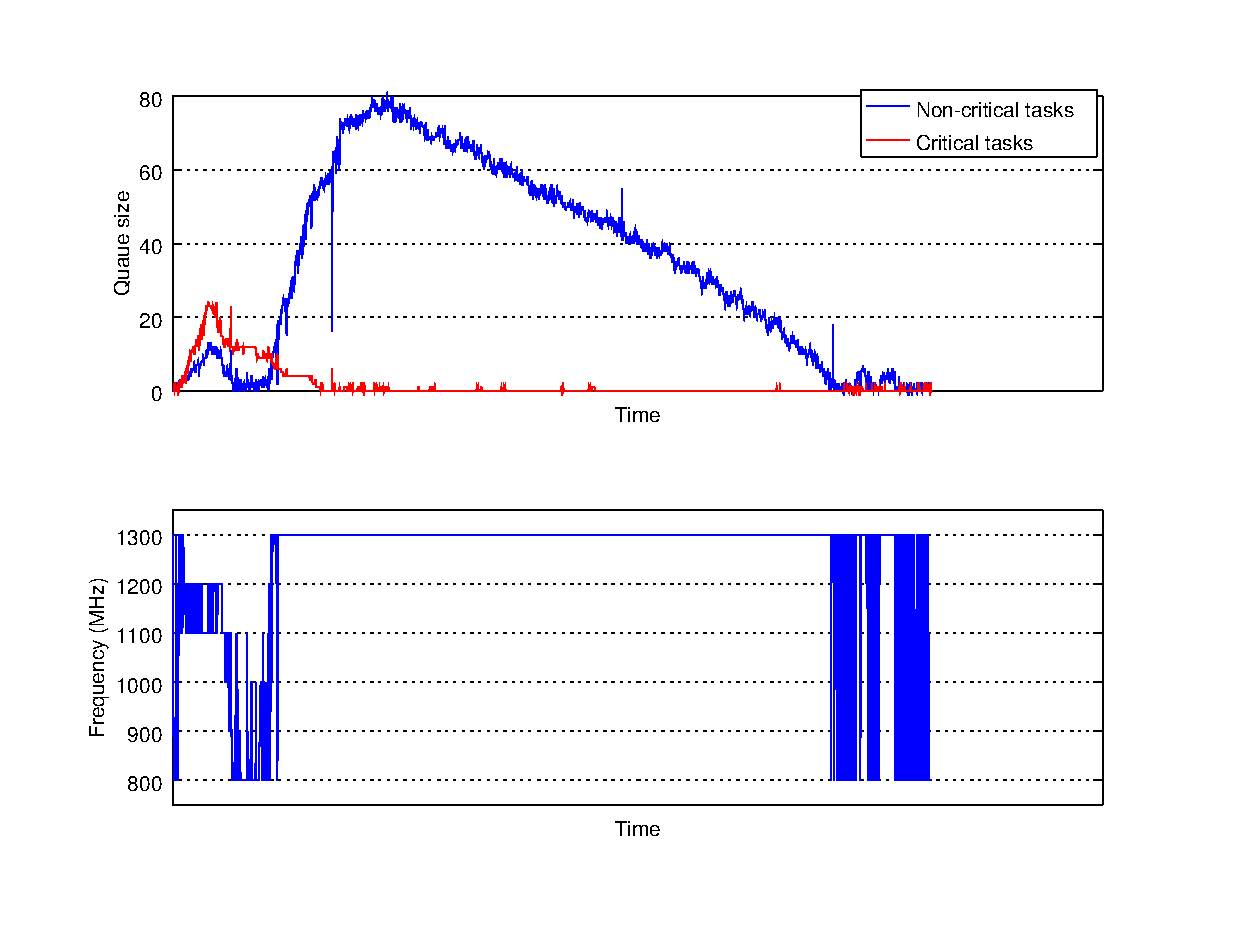
\includegraphics[width=1\textwidth]{Figures/Politicas_evo/P1_1024-64_juno.eps}}
  \caption[Cambio de frecuencias según la política P1]{Cambio de
    frecuencias según la política P1 para una factorización de Cholesky
    sobre una matriz de 1024 elementos dividida en bloques de 64, ejecutada
    sobre la plataforma \juno.}
  \label{s5:fig:P1-evo}
\end{figure}

\subsubsection{Políticas P2 y P2'}

A la hora de aplicar técnicas de escalado de frecuencia (DVFS) sobre un problema, la técnica
presenta de manera simplificada dos grandes dimensiones en las que tomar
decisiones sobre los parámetros de configuración para conseguir el objetivo
de reducir el consumo total: {\em (a)}~una primera dimensión que determina {\em qué
frecuencias utilizar} durante los diferentes cambios, y {\em (b)}~una segunda
dimensión que determina {\em en qué momentos de la ejecución se debe modificar
la frecuencia.}

La primera dimensión normalmente viene determinada por la propia arquitectura
sobre la que se ejecuta el problema, ya que es común que el procesador o el sistema operativo no
puedan seleccionar cualquier frecuencia de funcionamiento, sino solamente a una serie de
frecuencias predeterminadas. Esto hace que tomar la decisión de a
qué frecuencia se desea que el procesador trabaje se reduzca a 
una elección sobre un conjunto cerrado y finito de frecuencias. Cabe destacar que,
en ocasiones, puede resultar conveniente descartar algunas de estas frecuencias y
no tenerlas en consideración, ya sea porque impactan de manera muy negativa
en el rendimiento, o no tienen un impacto significativo en la mejora de
consumo.

La segunda dimensión está estrechamente relacionada con el problema a
ejecutar y el conocimiento que se tenga de él. Las decisiones que se pueden
tomar varían desde decisiones de grano grueso, como por ejemplo considerar 
el nivel de carga de trabajo de cada procesador y variar la frecuencia en
función de dicho parámetro, hasta decisiones de grano más fino, por ejemplo 
conocer el comportamiento de cada una de las tareas a ejecutar y el árbol
de dependencias de antemano, y así tomar decisiones en función de estos
parámetros. Por ejemplo, si una tarea es crítica, es posible aumentar la
frecuencia del núcleo asociado para así liberar nuevas tareas cuanto antes; o si se
sabe que la ejecución va a estar bloqueada hasta que no finalice una tarea
en concreto, es posible disminuir la frecuencia del resto de núcleos hasta que
esta tarea finalice, y así disminuir el consumo energético. Hay que
destacar que aunque disminuir la frecuencia del procesador implique conseguir
una potencia instantánea menor, esto no siempre implica que la energía final
consumida sea también menor: al bajar la frecuencia, el tiempo
empleado para finalizar la ejecución de una tarea puede aumentar lo
suficiente para provocar un consumo de energía mayor global. Por tanto,
cualquier decisión que afecte a la variación de frecuencia se debe considerar
como un compromiso entre rendimiento y consumo energético; la clave aquí radica
en optimizar dicho compromiso.

Adicionalmente a estas dos dimensiones, los sistemas heterogéneos en general, y
las arquitecturas asimétricas en particular, presentan una dimensión extra sobre
la que tomar decisiones: {\em (c)}~decidir {\em sobre qué elementos de cálculo} aplicar
el escalado de frecuencia. En el caso de las arquitecturas asimétricas,
esta decisión se reduce a decidir si aplicar el escalado de frecuencias
al cluster de núcleos \BIG, o al cluster de núcleos \LITTLE, dadas las limitaciones
en la selección de frecuencias mencionadas en la Sección~\ref{sec:DVFS_BIGLITTLE}.

La primera intuición que surge al intentar aplicar un escalado de
frecuencia sobre una arquitectura asimétrica es la de pensar que debido a
la gran diferencia de rendimiento entre los cores \BIG y \LITTLE (como 
muestra la Figura~\ref{fig:modelo_consumo}), aplicar una reducción de frecuencia a
los núcleos \BIG puede suponer una pérdida significativa de rendimiento, lo
cuál puede provocar incluso un aumento en el consumo energético al acarrear
un mayor tiempo global de ejecución; es decir, esta técnica podría llegar a
empeorar tanto el rendimiento como el consumo energético. Para evitar que
suceda este hecho, las políticas P2 y P2' han sido diseñadas para modificar
la frecuencia exclusivamente sobre el cluster de núcleos \LITTLE, con el fin de no causar
gran impacto sobre el rendimiento global. Además, las políticas han sido
desarrolladas sobre el planificador \botlev descrito en la
sección~\ref{s3:botlev}, con el objetivo de asegurar que las
tareas críticas se ejecutan en los núcleos \BIG y así evitar que estas
retrasen su ejecución si se ejecutaran en un núcleo \LITTLE con la frecuencia
disminuida.

Para determinar cuándo variar la frecuencia del cluster, las políticas P2 y P2' tiene en cuenta
el número de tareas listas para ser ejecutadas; así, si existen suficientes
tareas listas para ser ejecutadas, la frecuencia será alta para 
finalizar la ejecución cuanto antes, mientras que si existen pocas tareas
listas para ser ejecutadas, la frecuencia será menor, intentando favorecer
el ahorro energético. Este planteamiento es similar a tener en cuenta la
carga de trabajo del sistema, pero medida en número de tareas pendientes en
vez de ciclos ociosos/ocupados del procesador. Más concretamente, las
políticas monitorizan el tamaño de la cola de tareas listas para ser
ejecutadas, y determinan cuál es el tamaño máximo de la cola hasta el
momento de manera dinámica. Si la cola posee un tamaño igual o superior al
tamaño máximo conocido, significa que el número de tareas es elevado y por
tanto la frecuencia debe ser elevada. Si el tamaño es menor, entonces se
determina en que porcentaje es menor, y en función de las frecuencias
consideradas se toma la decisión de modificar la frecuencia actual o no. 

En la Figura~\ref{s5:fig:listing-p2} se muestra el pseudocódigo
asociado a estas políticas. El bloque \texttt{if} de la
línea~\ref{s5:lst:p2-detectPico} es el encargado de determinar si el tamaño
actual de la cola es mayor o igual que cualquier tamaño observado hasta el momento, y
en caso de ser así, configurar el cluster para que funcione a máxima
frecuencia. Esta comprobación es equivalente a determinar si hay un pico de carga de
trabajo. Las líneas~\ref{s5:lst:p2-tamStep1}-\ref{s5:lst:p2-tamStep2}
determinan el número de tareas que separan una frecuencia de la otra. La
forma de determinar esta cantidad consiste en repartir de manera equitativa
el espacio máximo de tareas conocido hasta el momento entre todas las
frecuencias, y asignar la frecuencia actual en función de qué tamaño posea
la cola (línea~\ref{s5:lst:p2-step}). Por ejemplo, si el cluster es capaz
de funcionar a 5 frecuencias distintas, y hasta el momento el número
máximo de tareas preparadas para ser ejecutadas ha sido de 20 tareas, antes
de cambiar de frecuencia se dispone de un margen de 4 tareas. Si el tamaño
actual de la cola es de 3 tareas, la frecuencia del cluster será la mínima,
mientras que si es de 5 tareas, la frecuencia será la frecuencia
inmeditamente superior a la frecuencia mínima.

\begin{figure}
  \centering

  \begin{lstlisting}[language=C++]
int P2(int littleQueueSize, int bigQueueSize){      
  //Comprobamos si estamos en un pico de carga
  if(littleQueueSize >= FreqCfg::maxQueueSize){ |\label{s5:lst:p2-detectPico}|
    FreqCfg::maxQueueSize = littleQueueSize;

    return changeLittleFreq(FreqCfg::maxLittleFreq);
  }

  //Tamanyo para cambiar de frecuencia
  float tamStep = (FreqCfg::maxQueueSize*1.0 /     |\label{s5:lst:p2-tamStep1}|
                   (FreqCfg::maxIdxLittle+1)*1.0); |\label{s5:lst:p2-tamStep2}|
  //Escalon actual
  int step = (int) (littleQueueSize / tamStep);    |\label{s5:lst:p2-step}|

  return changeLittleFreq(FreqCfg::littleFreqs[step]);
}
  \end{lstlisting}

  \caption{Pseudocódigo para las políticas P2 y P2'.}

  \label{s5:fig:listing-p2}
\end{figure}

La diferencia entre las políticas P2 y P2' radica en el rango de
frecuencias que se consideran para el cluster. Así, mientras la política P2
divide el tamaño de la cola entre todas las frecuencias posibles para el
cluster, la política P2' solamente considera la frecuencia máxima y mínima
del mismo.

\subsubsection{Política P3}

La política P3 es similar a la política anterior P2, pero realizando el
escalado de frecuencias sobre el cluster de núcleos \BIG en lugar de sobre los núcleos
\LITTLE. De manera similar a la anterior, la política ha sido implementada
sobre el planificador \botlev implementado en \ompss para 
minimizar el impacto negativo sobre las tareas críticas. La
Figura~\ref{s5:fig:P3-evo} muestra los distintos cambios de frecuencia que
se han realizado en función del número de tareas listas para ser
ejecutadas sobre un ejemplo concreto. En la gráfica superior se muestra la evolución del número de
tareas listas para ser ejecutadas según avanza la ejecución del problema,
mientras que en la gráfica inferior se muestra la frecuencia del cluster
\BIG durante la ejecución del problema. Ambas gráficas poseen la misma
escala en el eje x, permitiendo relacionarlas de manera visual. La gráfica
corresponde a una ejecución sobre la plataforma \juno para una factorización
de Cholesky sobre una matriz de $4608 \times 4608$ elementos dividida en bloques
de dimensión 512 en precisión simple.


\begin{figure}
  \centering
  {
    \setlength{\fboxsep}{-10pt}
    \fbox{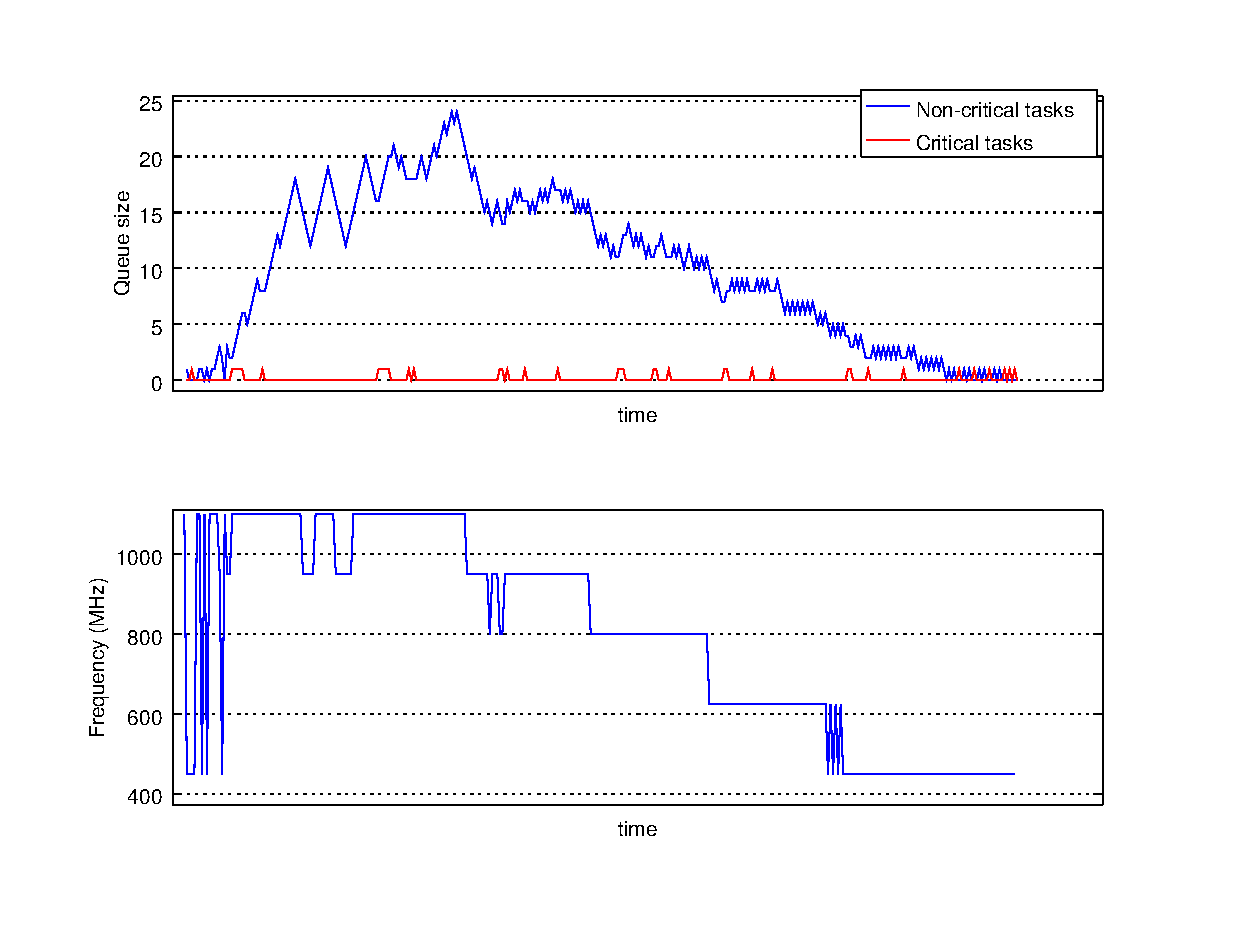
\includegraphics[width=1.0\textwidth]{Figures/Politicas_evo/P3_4608-512.eps}}
  }
  \caption[Escalado de frecuencia en función del número de tareas listas
  según la política P3]{Escalado de frecuencia en función del número de
    tareas listas según la política P3. La ejecución corresponde a una
    factorización de Cholesky sobre una matriz de 4608 elementos en
    precisión simple, dividida en bloques de tamaño de 512 elementos,
    ejecutada sobre la plataforma de desarrollo Juno (donde los cores big
    corresponden a cores ARM-A57).}
  \label{s5:fig:P3-evo}
\end{figure}


Como se puede observar en la gráfica, la ejecución se puede dividir en dos
partes bien diferenciadas: una primera parte hasta que alcanza la cola el
tamaño máximo, y una segunda parte en la que el número de tareas listas
desciende constantemente. Estas dos partes están totalmente relacionadas
con el grafo de dependencias de una factorización de Cholesky, donde existe
una primera fase en la que se crean un gran número de tareas y se expande
el árbol, y una segunda fase donde las tareas se van ejecutando y el árbol
se cierra paulatinamente.

Debido a que el cálculo del tamaño máximo de la cola se realiza de manera
dinámica, en la primera fase se realizan cambios de frecuencia
continuamente a causa de ligeros cambios en el tamaño de la cola hasta que
se consigue estabilizar la cota superior, y poder aplicar la política de
manera correcta. Una vez alcanzado el tamaño máximo de la cola, se observa
como el espacio está dividido en varios escalones, cada uno correspondiente
a una frecuencia distinta, y según el tamaño de la cola va disminuyendo y
cambiando de escalón, las frecuencias son modificadas. Puede darse el caso
en el que el tamaño de la cola esté variando continuamente entre dos
escalones, produciendo que la frecuencia oscile hasta que el tamaño de la
cola se vuelva a estabilizar. Esta situación se puede apreciar al principio
del escalón asociado a 950MHz, donde se aprecia como un ligero descenso del
número de tareas produce que la frecuencia oscile entre 800MHz y 950MHz.


\subsection[Basadas en planificación de tareas (P4, P5 y P6)]{Basadas en planificación de tareas}

\subsubsection{Políticas P4 y P5}

Las políticas descritas hasta el momento intentan obtener una mejora en el
rendimiento energético a partir de un escalado de frecuencia en los
distintos clusters de la arquitectura, prestando atención al número de
tareas listas para ser ejecutadas como medida equivalente a detectar el
nivel de carga de trabajo en un cierto momento. Estas políticas se han
desarrollado prestando atención a la Figura~\ref{fig:modelo_consumo}, en la
que se puede observar la disminución del consumo energético en función de
la frecuencia. La siguiente idea que surge prestando atención a la misma
figura consiste en disminuir el consumo al no utilizar algún cluster
durante parte de la ejecución. Como se puede observar, el consumo energético
es menor si el cluster presenta carga, independientemente de la frecuencia
utilizada. Las siguientes políticas han sido diseñadas con el objetivo de
que, en ciertos momentos de la ejecución, se evite asignar tareas a cierto
cluster del sistema, modificando el planificador de tareas.
Es decir, estas políticas no están orientadas a realizar técnicas de escalado
de frecuencia, sino que tratan con el
problema de planificación de tareas a los distintos \wts disponibles.

La política P4 monitoriza el tamaño de las colas de tareas listas y, en
función del tamaño de la cola respecto al tamaño máximo (similar a la
política P2 o P3), decide si asignar tareas listas al cluster de cores
\LITTLE o por el contrario no hacerlo. En caso de que el tamaño de la cola 
sea lo suficientemente pequeño, la política no asigna ninguna tarea lista al cluster, provocando
que este se encuentre ocioso. Cabe destacar que, aunque el planificador
no asigne tareas al cluster, esto no implica que el sistema operativo no
ejecute procesos sobre él; aún así, según se ha observado, el impacto final 
sobre el consumo energético es mínimo comparado con el de ejecutar una tarea.

Para realizar este proceso, cada vez que una tarea se inserta en la cola de
tareas listas o es extraída de ésta, se compara el tamaño actual de la cola
con el tamaño máximo conocido hasta el momento, y se decide si se debe
utilizar el cluster o no para ejecutar tareas. Una vez que un \wt
finaliza la ejecución de una tarea, éste solicita una nueva tarea a
ejecutar al planificador. Si el \wt se ejecuta sobre un núcleo del cluster
\LITTLE, y se ha decidido que el cluster no ejecute ninguna acción, al \wt
se le asigna una tarea nula, evitando así la ejecución de cualquier tarea
en ese core asociado al \wt y perteneciente al cluster inhabilitado. En
caso de que el cluster no se encuentre desactivado se asigna la siguiente
tarea de la cola de tareas listas para que la ejecute el \wt.

Para que esta política funcione correctamente, es necesario que se verifiquen algunas
condiciones cuando se ejecute el problema:

\begin{itemize}
\item El número de \wts lanzados debe coincidir con el número de núcleos del
  SoC. En caso de que el número de \wts sea superior, varios \wts
  competirían por ejecutarse simultáneamente en el mismo núcleo. De manera
  contraria, si el número de \wts es menor que el número de núcleos, se
  estarían desaprovechando recursos ya que no se utilizarían todos los
  núcleos de manera simultánea. En \nanos esto se consigue mediante el
  argumento \texttt{--smp-workers=<n>}.
\item Cada \wt debe estar asignado a un núcleo único de la placa,
  provocando que un \wt siempre ejecute tareas en el mismo núcleo durante
  todo el problema. Esta condición unida a la anterior implica que existe
  una relación directa ({\em afinidad}) entre cada núcleo y cada \wt del
  \emph{runtime}.
\item Aunque se tenga control sobre qué tarea se ejecuta en qué \wt (y por
  tanto en qué núcleo), existen ciertas tareas pertenecientes al propio
  \emph{runtime} o al código no paralelo del programa sobre el que no se
  puede tomar decisiones desde el planificador, siendo normal que este
  código se ejecute sobre el \wt principal, normalmente ejecutado sobre el
  núcleo 0 de la máquina.
\end{itemize}


En las políticas anteriores, donde se disponía un número limitado de
frecuencias, el punto en el que cambiar la frecuencia venía determinado a
la hora de repartir por igual el tamaño máximo de la cola entre todas las
frecuencias disponibles. Para dar mayor flexibilidad a esta política, el
punto en el que tomar la decisión de apagar el cluster viene determinado
por una variable de entorno elegida por el usuario a la hora de lanzar el
experimento. Esto permite observar el comportamiento variando el momento en
el que se desactiva el cluster, como se describe en la siguiente
sección. Además, para evitar efectos rebote, en los que el cluster se esté
activando y desactivando de manera continuada, mediante experimentación se
ha decidido insertar un margen del 10\% del tamaño de la cola antes de
tomar la decisión de apagar o encender el cluster.

La Figura~\ref{fig:P4-puedo-ejecutar} muestra un fragmento del código
encargado de determinar si un \wt debe ejecutar una tarea lista o no. La
función recibe por parámetro el núcleo al que se encuentra asignado el \wt
y devuelve un valor \emph{booleano} en función de si el cluster se
encuentra desactivado o no. Para agilizar el proceso, la
línea~\ref{lst:p4-a} filtra la ejecución y permite continuar con la
ejecución únicamente en el caso de que el cluster se encuentre
desactivado. La labor de determinar si el cluster debe estar activo o no se
realiza en el momento en el que una tarea lista es insertada en la cola de
tareas listas, o es extraída, y se realiza mediante un código similar
al de la Figura~\ref{s5:fig:listing-p2}. Si el cluster se encuentra
desactivado, mediante las siguientes líneas se determina si el núcleo
pertenece al cluster inactivo. En caso de pertenecer, se devuelve el
valor de falso para indicar que el \wt no debe ejecutar tareas, y además
se reduce la frecuencia de núcleo al mínimo para intentar minimizar el
consumo energético mientras no se utilice el cluster de cores \LITTLE
(línea~\ref{lst:p4-c}).


\begin{figure}
  \centering
\begin{lstlisting}[language=C++]
bool CoresCfg::puedoEjecutar(int coreId){
  //core little
  if(apagadoLittle)                     |\label{lst:p4-a}|
    for(int i=0; i<N_CORE_LITTLE; i++)
      if(coresLittle[i] == coreId){     |\label{lst:p4-b}|
        if (!coresApagados[coreId]){
          FreqCfg::changeLittleFreq(FreqCfg::minFreqLittle); |\label{lst:p4-c}|
          coresApagados[coreId] = true;   |\label{lst:p4-d}|
        }
        return false;
      }
\end{lstlisting}
  \caption{Fragmento de código para determinar si asignar una tarea a un
    \wt o no.}
  \label{fig:P4-puedo-ejecutar}
\end{figure}

La política P5 realiza el mismo procedimiento, pero para el cluster de
núcleos \BIG. Ambas políticas están implementadas sobre el planificador \botlev
para así asegurar que la ejecución de tareas críticas siguen siendo en
núcleos \BIG. Sin embargo, al desactivar los núcleos \BIG, hay que tener en cuenta
que es necesario que las tareas críticas se ejecuten ahora en núcleos \LITTLE si los
\BIG no están disponibles para que la ejecución no se quede bloqueada por
las tareas críticas (la opción \texttt{--steal=1} en \botlev activa el {\em work-stealing}
en \nanos).

La Figura~\ref{fig:P4-evo} muestra un ejemplo de esta política para la
ejecución de una factorización de Cholesky. La gráfica superior muestra la
ejecución de las diferentes tareas por los distintos \wts, cada uno
asignado a un núcleo distinto en orden de aparición. La ejecución ha sido
realizada sobre la plataforma \juno, por lo que los 4 primeros núcleos
corresponden a núcleos \LITTLE, mientras que los dos siguientes a núcleos
\big. La segunda gráfica muestra la evolución del tamaño de las colas en
función del tiempo. Como se puede observar, la ejecución de las tareas se
realiza de manera convencional hasta que el tamaño de la cola decrece por debajo
del 25\% del tamaño máximo (en este caso, el experimento se configuró con este valor
con fines meramente ilustrativos). En ese momento, los núcleos \LITTLE dejan de recibir tareas mientras que los \BIG
continúan su ejecución habitual. Una vez que el número de tareas vuelve a
incrementarse, los cores lentos vuelven a activarse y a ejecutar tareas,
hasta que al final de la ejecución el tamaño de la cola vuelve a decrecer
y el cluster se desactiva hasta finalizar la ejecución. Aunque el primer
\wt está asociado a un núcleo \LITTLE, también es considerado como el \wt
principal del planificador, por lo que es el encargado de ejecutar la parte
del código no paralela (en color verde). La mayor parte del tiempo que se
encuentra ejecutando este código corresponde a tareas del propio
planificador, o a la espera de que finalice la ejecución paralela (marcada
por una etiqueta \texttt{\#pragma omp taskwait} en el código secuencial),
por lo que el impacto final sobre el consumo energético no es significativo.

\begin{figure}
  \centering
  \begin{framed}
    \begin{subfigure}{1\textwidth}
      \centering
      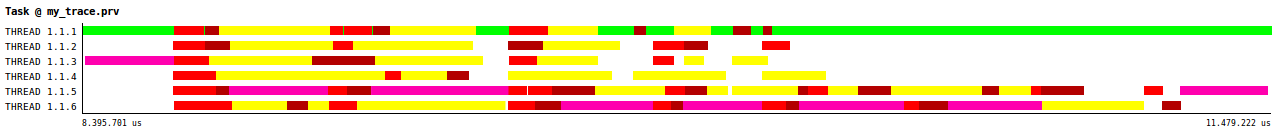
\includegraphics[width=1\linewidth]{Figures/Politicas_evo/Apagado_tareas.png}
      \caption{Asignación tareas a los distintos \wts.}
      \label{}
    \end{subfigure}

\vspace{0.5cm}

    \begin{subfigure}{1\textwidth}
      \centering
      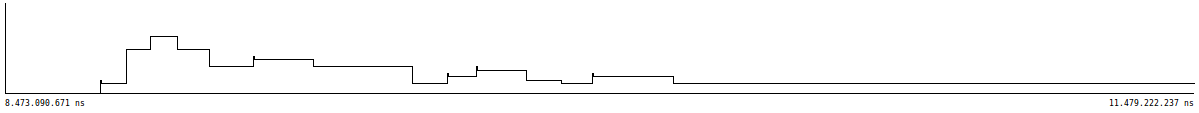
\includegraphics[width=1\linewidth]{Figures/Politicas_evo/Apagado_colas.png}
      \caption{Evolución del tamaño de la cola de tareas listas.}
      \label{}
    \end{subfigure}  
    
    % \begin{subfigure}{0.9\textwidth}
    %   \centering
    %   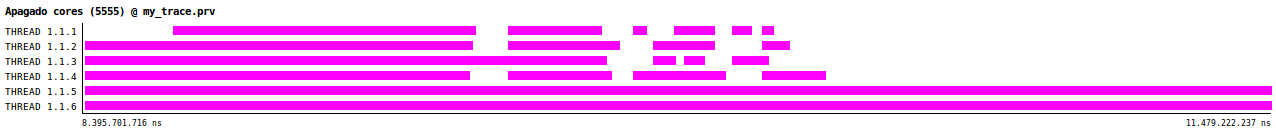
\includegraphics[width=1\linewidth]{Figures/Politicas_evo/Apagado_cores.png}
    %   \caption{Estado de los núcleos. Rosa = activo. Blanco = inactivo.}
    %   \label{}
    % \end{subfigure}  
  \end{framed}
  \caption[Asignación de tareas en función del tamaño de la cola según la
  política P4]{Asignación de tareas en función del tamaño de la cola según
    la política P4. La gráfica superior muestras las distintas tareas
    ejecutadas por cada uno de los \wts a lo largo del tiempo. Clave de
    colores: rojo=\trsm, rosa=\potrf, granate=\syrk, amarillo=\gemm,
    verde={\sc main}. La ejecución corresponde a una factorización de
    Cholesky para una matriz de 4096 elementos dividido en bloques de
    tamaño 512 en precisión simple sobre una arquitectura \juno, donde los
    4 primeros \wts corresponden a los cores lentos y los 2 últimos a los
    cores rápidos. La política está configurada para desactivar cores a
    partir del 25\% del tamaño máximo de la cola.}
  \label{fig:P4-evo}
\end{figure}



\subsubsection{Política P6}
\label{sec:p6}

Una de las muchas funcionalidades que ofrece el kernel Linux es la de poder
activar y desactivar núcleos bajo demanda y de manera dinámica. En cualquier
momento de la ejecución, un núcleo puede ser desactivado, y este desaparece
del sistema, siendo totalmente transparente para cualquier aplicación en
ejecución. Esto implica que si se decide apagar un núcleo, todos los procesos
asociados a ese núcleo son migrados a otro de manera totalmente
transparente al proceso en ejecución, el número total de cores disminuye y
cualquier llamada a una función del kernel considerará la nueva
configuración hardware creada como la configuración real de la
máquina. Esta funcionalidad permite, por ejemplo, generar dinámicamente
arquitecturas diferentes utilizando el mismo hardware.

Esta funcionalidad aplicada a una arquitectura big.LITTLE teóricamente
conlleva que en cualquier momento de la ejecución se pueda desactivar
uno de los dos cluster de la máquina, convirtiendo la arquitectura en una
plataforma totalmente simétrica \footnote{En la práctica, no todas las versiones
del kernel permiten apagar el núcleo 0, por lo que en estos casos, no es posible apagar el
completametne el cluster que contiene a este núcleo}.

Para realizar un estudio del efecto del apagado selectivo de núcleos sobre el
consumo energético, se ha realizado el experimento de desactivar, uno a uno,
los núcleos de un mismo cluster mientras se monitoriza el consumo. Además, para
evitar errores en las medidas, se ha establecido un tiempo de espera entre
apagado de dos núcleos, y adicionalmente se ha ejecutado el test de carga asociado a
un núcleo que no se fuera a apagar, evitando así problemas al migrar el
proceso de un núcleo a otro. La Figura~\ref{s5:fig:apagadoCores} muestra las
mediciones del consumo energético en las dos plataformas: 
\juno (gráfica superior) y \odroid (gráfica inferior).

\begin{figure}
  \centering
  \begin{subfigure}{0.9\textwidth}
    \centering
    \fbox{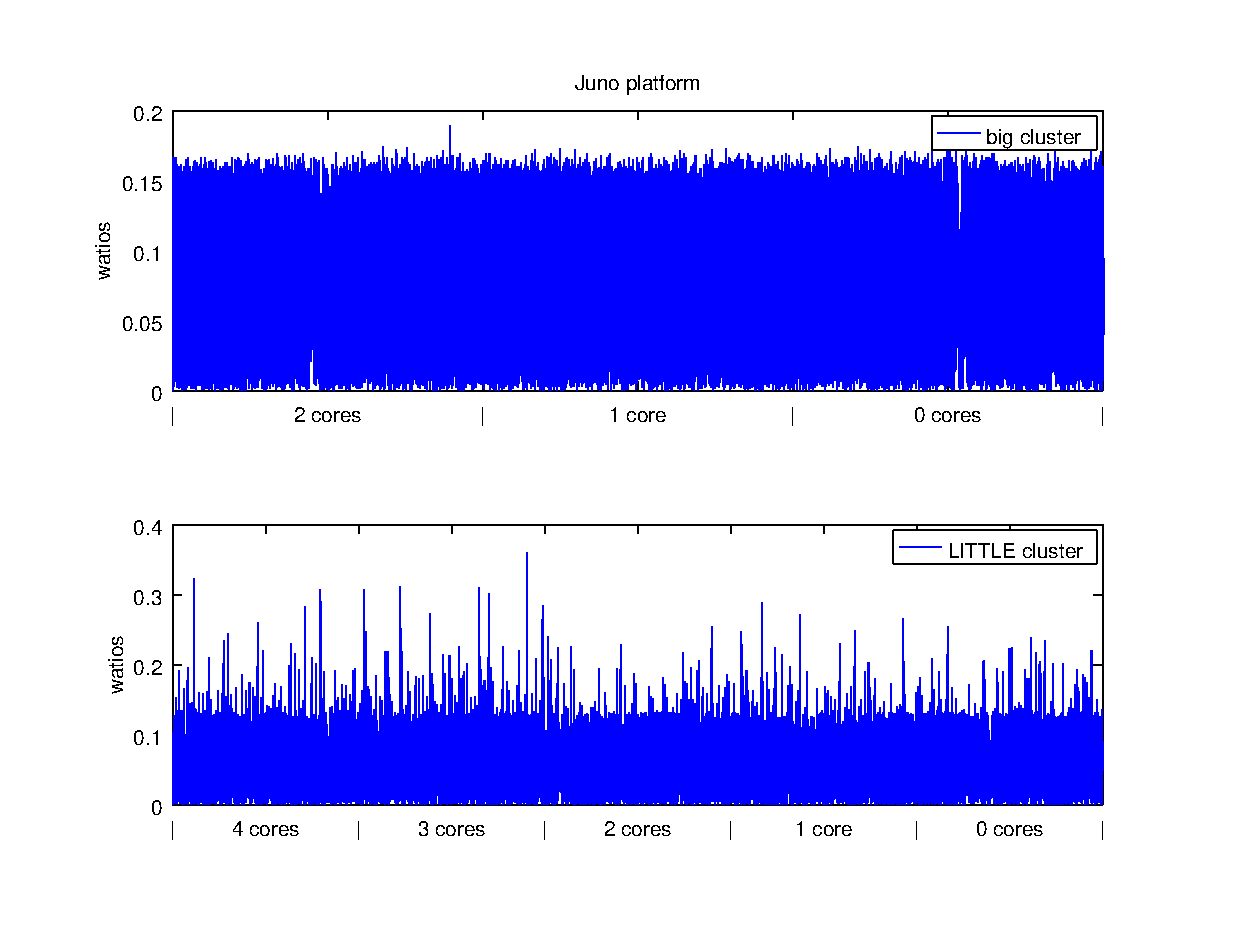
\includegraphics[width=0.75\linewidth]{Plots/Modelos_consumo/apagadoJuno.eps}}
    \caption{Plataforma \juno: 2 núcleos \BIG A57 y 4 núcleos \LITTLE A53.}
      \label{}
    \end{subfigure}

    \vspace{0.5cm}

    \begin{subfigure}{0.9\textwidth}
      \centering
      \setlength{\fboxsep}{20pt} %No tienen el mismo margen :(
      \fbox{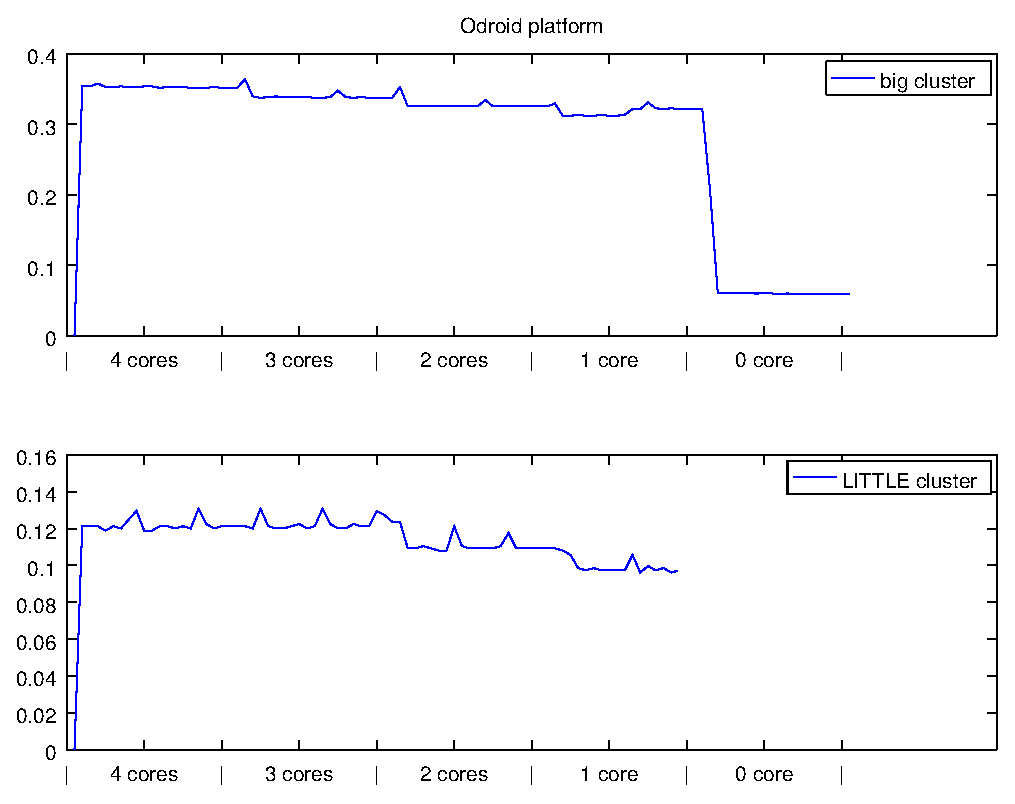
\includegraphics[width=0.66\linewidth]{Plots/Modelos_consumo/apagadoOdroid.eps}}
      \caption{Plataforma \odroid: 4 núcleos \BIG A15 y 4 núcleos \LITTLE A7.}
      \label{}
    \end{subfigure}  
    
  \caption[Consumo energético en función del número de cores activos en
  cada cluster]{Consumo energético en reposo en función del número de núcleos
    activos del sistema y de la plataforma. La versión del kernel Linux
    instalada en la plataforma \odroid no permite apagar los el cluster
    \LITTLE de manera completa.}
  \label{s5:fig:apagadoCores}
\end{figure}

Las gráficas muestran la potencia instantánea observada (en Watios) durante todo el
experimento en el eje vertical, mientras que el eje horizontal corresponde
a las distintas fases por las que ha ido pasando el experimento. Por cada
plataforma, la gráfica superior muestra el experimento apagando los cores
del cluster \BIG, indicándose en el eje x el número de núcleos activos del
cluster en cada momento; la gráfica inferior muestra el mismo
experimento para el cluster \LITTLE. La diferencia de aspecto entre las
gráficas de ambas plataformas se produce por la forma en la que se han
realizado las medidas: mientras que en la plataforma \odroid los medidores
poseen una frecuencia de muestreo máxima de 4 muestras por segundo (y por
eso el aspecto \emph{lineal} de la gráfica), el entorno de medición de la
plataforma \juno permite una mayor frecuencia de muestreo, por lo que la
gráfica presenta un mayor ruido (esta es la causa de que la gráfica no
presente una forma de línea, sino que los valores oscilan por encima y
debajo del valor medio real).

Observando los resultados de las gráficas se pueden extraer las siguientes
conclusiones:

\begin{enumerate}
\item En la plataforma \juno, desactivar cores es equivalente a no usarlos
  en lo referente al consumo energético.
\item Mientras que la versión del kernel Linux utilizada en la plataforma
  \juno permite apagar todos los cores del sistema, la versión utilizada en
  la plataforma \odroid no permite apagar el núcleo 0, por lo que no es
  posible desactivar el cluster \LITTLE completo.
\item En la plataforma \odroid, desactivar un cierto número de núcleos sin
  llegar a desactivar el cluster completo no tiene ningún impacto
  significativo en el consumo energético. Sin embargo, para esta
  plataforma, desactivar todos los núcleos del cluster \BIG conlleva que 
		la potencia instantánea caiga a niveles prácticamente nulos.
\end{enumerate}


Aprovechando la caída de pontencia cuando el cluster de
núcleos \BIG se desactiva por completo en la plataforma \odroid, la política
P6 ha sido desarrollada como una modificación de la política anterior, pero
además de no asignar tareas a estos cores, realiza un apagado controlado de
los mismos. Para realizar esta modificación, el cambio introducido sobre el
código de la Figura~\ref{fig:P4-puedo-ejecutar} afecta a la
línea~\ref{lst:p4-c}, en la que en vez de disminuir la frecuencia del
cluster, se realiza una llamada al código encargado de realizar el apagado
de los distintos núcleos, mostrado en la
Figura~\ref{s5:fig:apagadoCores}. Como se puede observar, el apagado del
núcleo se realiza escribiendo el valor 0 en el fichero del sistema ({\sc sysFS}) que se
encuentra en la ruta
\texttt{/sys/devices/system/cpu/cpu<cpuId>/online}. Esta operación se ha protegido
mediante un cerrojo para evitar problemas de concurrencia
durante la ejecución.



\begin{figure}
  \centering
\begin{lstlisting}[language=C++]
char path[50];
sprintf(path, "/sys/devices/system/cpu/cpu%d/online", coreId);

FILE* f;
int d, a;

(CoresCfg::_lock[coreId])->acquire();
{
  f = fopen(path, "r+");
  a = fscanf(f, "%d", &d);
	
  if(d!=0 && a!=0){
    fseek(f, 0, SEEK_SET);
    fprintf(f, "0"); //Apagado
  }
	
  fclose(f);
}
(CoresCfg::_lock[coreId])->release();
\end{lstlisting}
  \caption{Fragmento de código para el apagado de cores de manera
    dinámica.}
  \label{fig:lst:apagado-cores}
\end{figure}





\section{Resultados experimentales}

\subsection{Análisis de la mejora energética para las políticas P1-P3}

El primer conjunto de experimentos que se muestran a continuación tiene
como objetivo principal comprobar el nivel de eficiencia energética desde
la política P1 hasta la política P3, las cuales corresponden a políticas
que siguen una estrategia puramente DVFS como se ha descrito
anteriormente\footnote{En este capítulo todos los experimentos han sido
  realizados utilizando precisión simple.}. Los experimentos corresponden a
distintas ejecuciones de una factorización de Cholesky para distintas
configuraciones de tamaño de matriz y bloque. Para comprobar si estas
políticas presentan una mejora energética real, los resultados son
comparados con una ejecución convencional utilizando el planificador \botlev sobre
el \emph{runtime} \ompss (esta ejecución se denomina P0 en los experimentos
realizados). Para poder observar el comportamiento con detalle y poder
extraer mejores conclusiones, de todos los experimentos se extraen las tres
siguientes medidas:
\begin{enumerate}
\item Rendimiento computacional medido en GFLOPS\footnote{1 GFLOP equivale a $1e9$ operaciones en 
		punto flotante por segundo.}. Distintos rendimientos
  sobre la misma configuración del problema sirven para indicar
  diferencias en el tiempo de ejecución.

\item Muestreo de la potencia media (en Watios). Los medidores
  permiten extraer el muestreo de potencia diferenciado por clusters, aunque
		en este caso se muestra agregada para ambos cluster.

\item Eficiencia o rendimiento energético medido en GFLOPS/Watio, como resultado de
  combinar las dos medidas anteriores.
\end{enumerate}

En las Figuras~\ref{fig:resultados:all-0-3:juno}~y~\ref{fig:resultados:all-0-3:odroid}
se muestran de manera conjunta los resultados obtenidos para la plataforma
\juno y para la plataforma \odroid, respectivamente. Las gráficas
representan de manera conjunta las tres métricas mencionadas anteriormente
para las políticas P1 a P3 para un amplio conjunto de tamaños de matriz y
bloque.

A grandes rasgos, es posible extraer un conjunto de observaciones generales:

\begin{itemize}
\item Atendiendo exclusivamente al tamaño de problema, se pueden distinguir 
	dos grupos bien diferenciados: un primer grupo
  formado por las matrices de tamaño pequeño ($m \le 2048$), y un segundo
  grupo formado por las matrices de mayor tamaño. La principal diferencia
  radica en el rendimiento de las distintas políticas respecto a la
  ejecución normal sobre \botlev: mientras que en el segundo grupo el
  rendimiento se aproxima al de una ejecución normal con \botlev (aunque
  casi siempre inferior), en el primer grupo la diferencia de rendimiento
  es muy elevada, siempre a favor de \botlev. Esta diferencia provoca no solo un rendimiento
  computacional menor, sino una eficiencia energética considerablemente
  inferior. Además, hay que destacar que esta diferencia es más elevada en
  la plataforma \odroid que en la plataforma \juno.
\item El comportamiento de todas las políticas es similar en ambas
  plataformas, dando una mayor validez a los datos. Además, la proporción
  entre el número de núcleos \BIG y \LITTLE varía entre una plataforma y otra,
  dando mayor relevancia a los datos.
\item Mientras que las políticas P1, P2 y P2' obtienen un rendimiento
  energético muy similar a la ejecución convencional sin aplicar ninguna
  política, la política P3 obtiene un rendimiento energético mucho mayor
  que la ejecución con \botlev sobre \ompss.
\end{itemize}  

\comentario{Rehacer gráfica para aprovechar el espacio}
\begin{figure}
  \centering
  \fbox{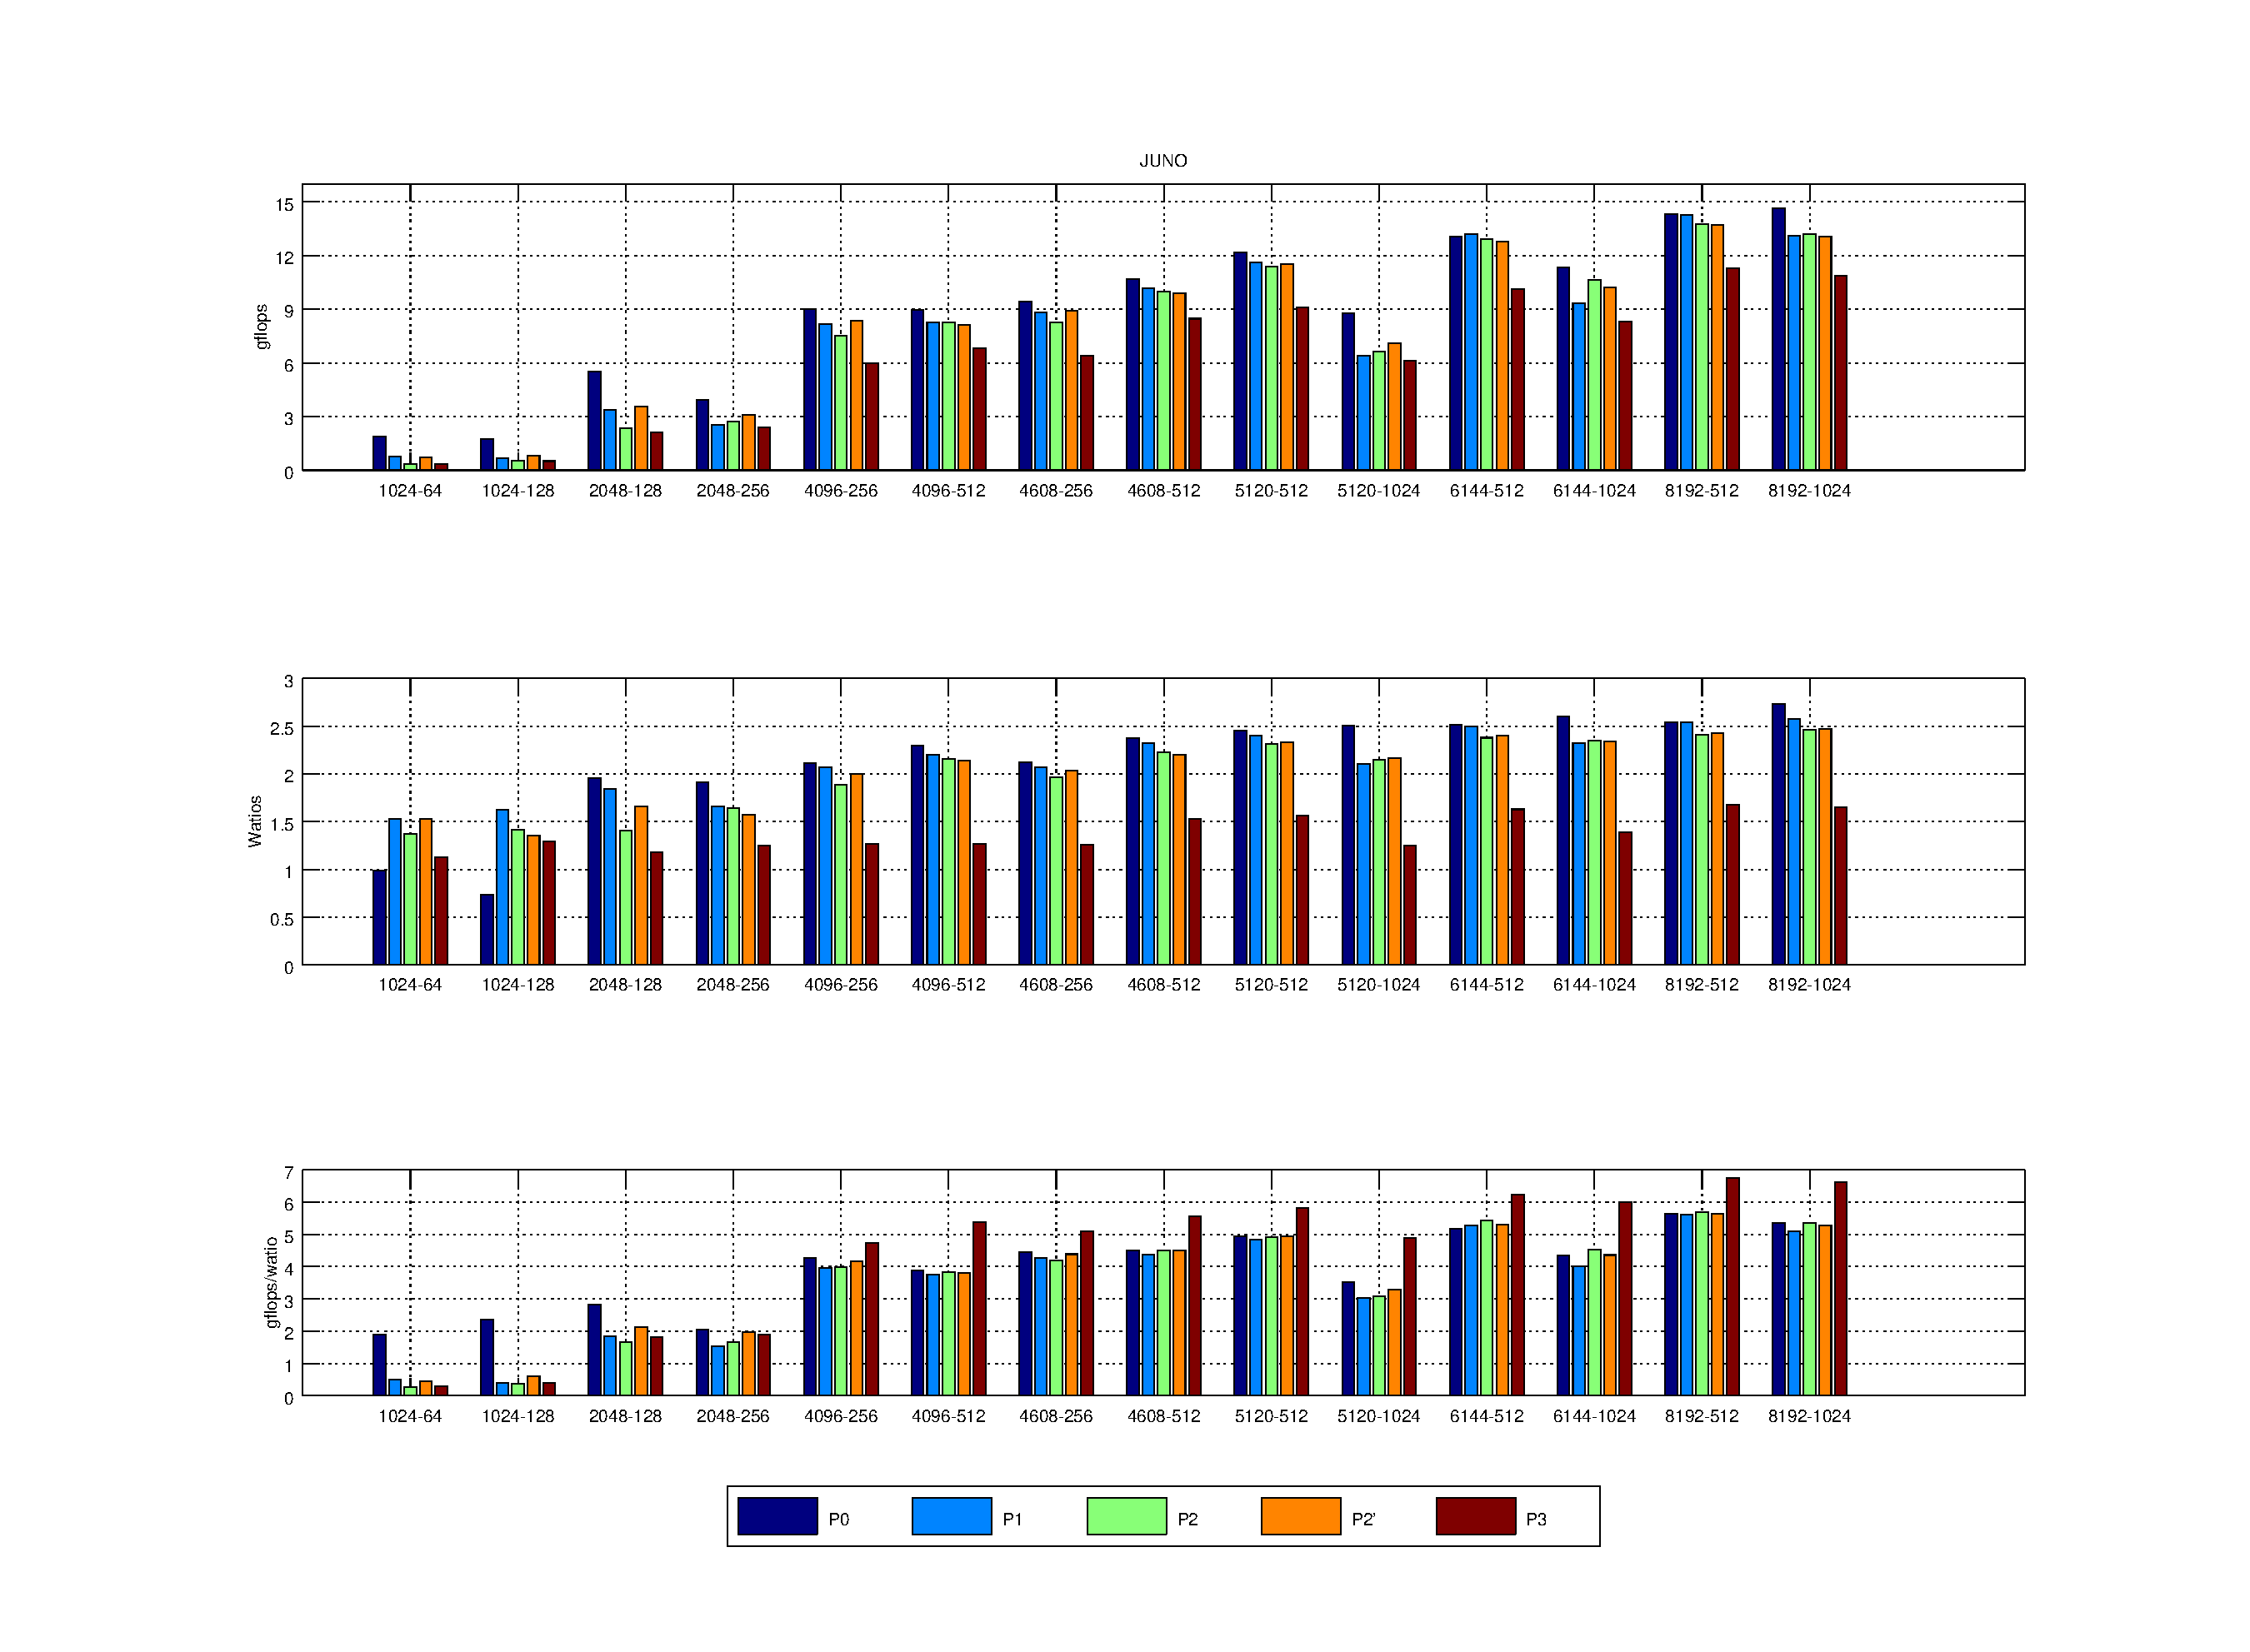
\includegraphics[width=1.0\textwidth]{Plots/dvfs_results/0-4_all_juno.eps}}
  
  \caption[Medidas experimentales para las políticas desde P1 a P3 en \juno]{Medidas
    experimentales para las políticas desde P1 a P3 para la plataforma \juno. La política P0
    representa a una ejecución normal con \botlev. Las etiquetas del eje x
    representan el tamaño de la matriz y de bloque utilizado para el experimento.}
  \label{fig:resultados:all-0-3:juno}
\end{figure}

\begin{figure}
  \centering
  \fbox{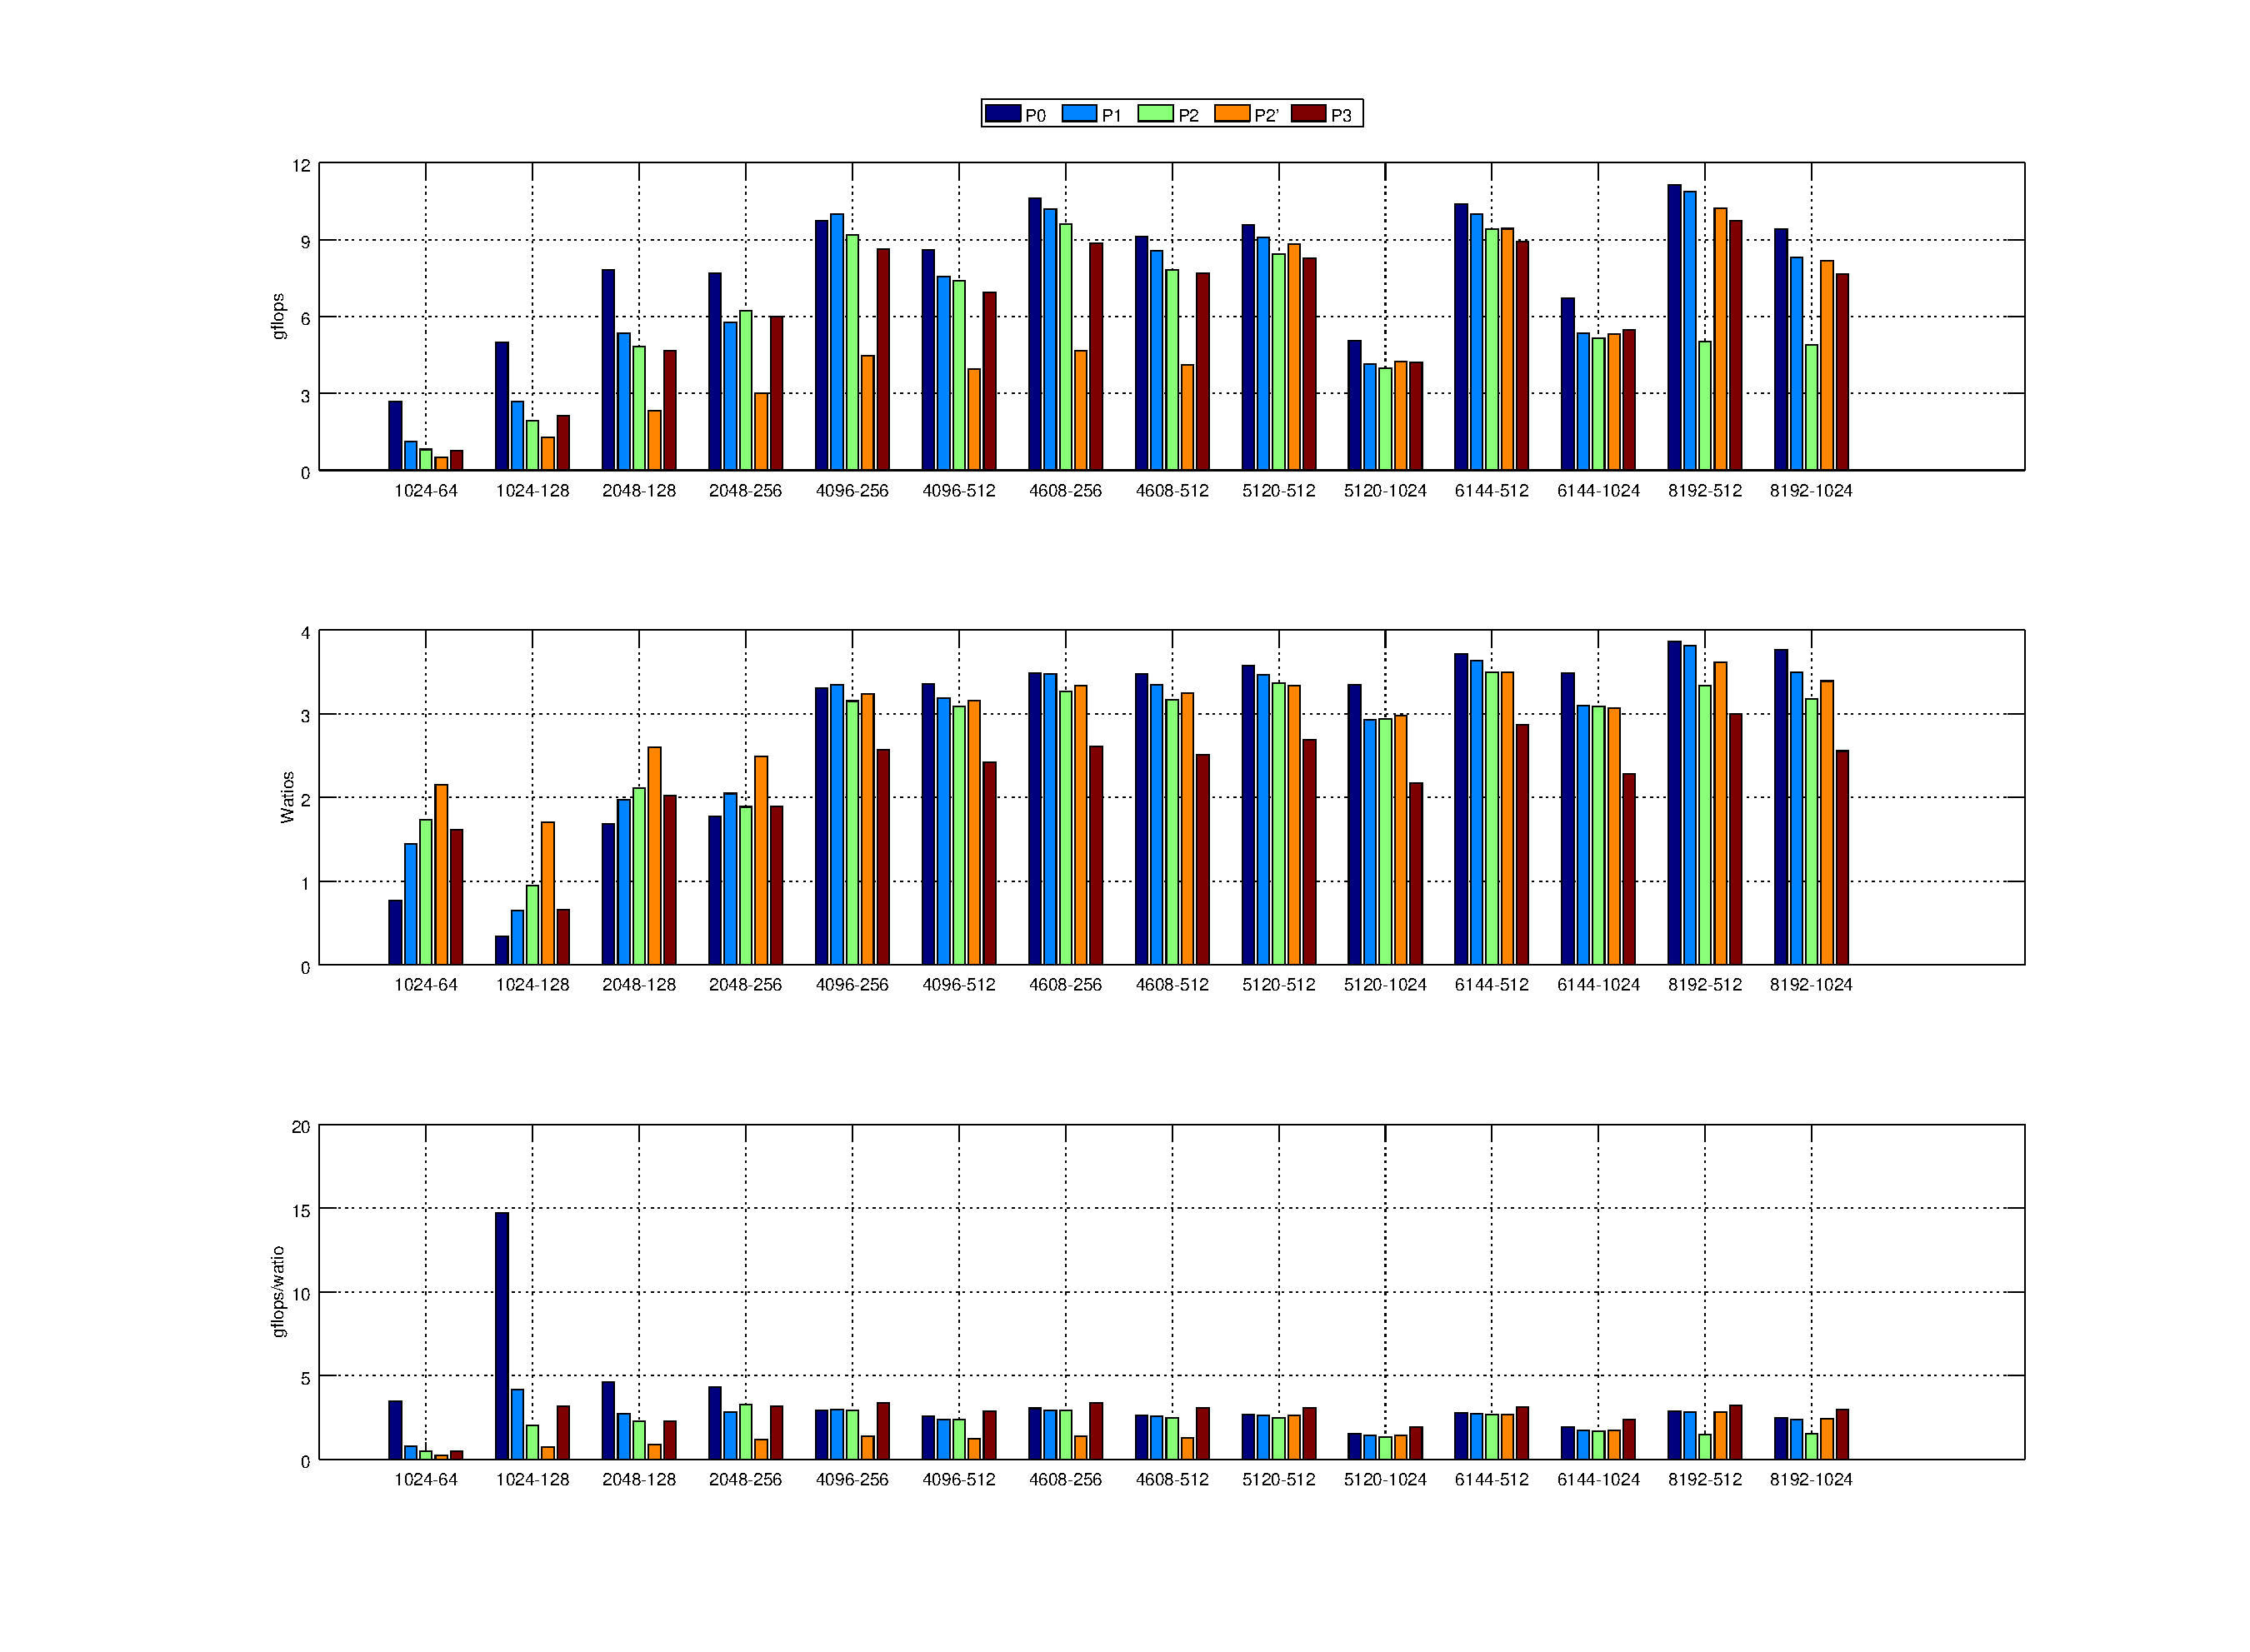
\includegraphics[width=1.0\textwidth]{Plots/dvfs_results/0-4_all_odroid.eps}}
  \caption[Medidas experimentales para las políticas desde P1 a P3 en \odroid]{Medidas
    experimentales para las políticas desde P1 a P3 en la plataforma \odroid. La política P0
    representa a una ejecución normal con \botlev. Las etiquetas del eje x
    representan el tamaño de la matriz y de bloque utilizado para el experimento.}
  \label{fig:resultados:all-0-3:odroid}
\end{figure}

Prestando más atención a la política P1, se observa que no presenta una
gran diferencia respecto a la ejecución convencional utilizando \botlev. La causa de este
hecho está relacionada con el DAG asociado a la factorización de Cholesky,
el cual se caracteriza por una rápida explosión de tareas al comienzo de la
ejecución, provocando que el número de tareas críticas sea inferior al
número de tareas no críticas durante casi toda la ejecución. Como trabajo
futuro se considera experimentar esta política sobre otros problemas donde
su DAG se abra y cierre sucesivamente durante la ejecución.

Respecto a las políticas P2 y P2', no presentan una gran diferencia entre
ellas en los resultados, tanto en el rendimiento en GFLOPS, como el consumo
de energía. La razón de este parecido radica en que las políticas son
prácticamente iguales, únicamente variando el conjunto de frecuencias sobre
las que elegir para realizar el escalado de frecuencia. Respecto a la
mejora del rendimiento energético, que es el objetivo final buscado, no se
consigue superar el rendimiento alcanzado por una ejecución normal de
\botlev; sin embargo, se observa que la potencia instantánea media consumida
ha disminuido. Este dato, junto con el hecho de que el rendimiento
energético (GFLOPS/watio) no disminuye considerablemente respecto a la
ejecución normal, hacen que las políticas P2 y P2' representen una posible
solución para arquitecturas cuya potencia instantánea máxima está limitada
por motivos de diseño o por el entorno de ejecución (por ejemplo, sistemas
alimentados por baterías). La Tabla~\ref{tab:mejora-potencia} representa la
disminución de potencia en watios respecto a la ejecución normal de
\botlev. Como se puede observar, salvo el primer grupo de matrices que
identificábamos anteriormente, el resultado es bueno para todas las políticas,
obteniendo disminuciones de potencia cercanas a 0.25 watios para las
políticas P2 y P2', y reducciones de hasta 1 watio para la política P3
sobre la plataforma \juno.

%%% WATIOS %%%%
\begin{table}
  \centering
  \caption{Mejora de la potencia instantánea media para las políticas P1-P3.}
  \label{tab:mejora-potencia}
  {\scriptsize
    \begin{tabular}{cccccccccccccccc}
      \toprule
      \multicolumn{2}{c}{\phantom{a}} & \multicolumn{14}{c}{Tamaño de la matriz \texttt{(m)} y
                                        de bloque \texttt{(b)}.} \\ \cmidrule{2-16}
      \phantom{4} & \texttt{(m)} & \multicolumn{2}{c}{1024} & \multicolumn{2}{c}{2048} &                                                                         \multicolumn{2}{c}{4096} & \multicolumn{2}{c}{4608} & \multicolumn{2}{c}{5120} & \multicolumn{2}{c}{6144} & \multicolumn{2}{c}{8192} \\
      \phantom{a} & \texttt{(b)} & 64 & 128 & 128 & 256 & 256 & 512 & 256 & 512 & 512 & 1024 & 512 & 1024 & 512 & 1024 \\ \hline

      {\sc P1} & \phantom{a} & \br{-0.538} & \br{-0.897} & \fg{0.118} & \fg{0.260} & \fg{0.040} & \fg{0.100} & \fg{0.053} & \fg{0.054} & \fg{0.051} & \fg{0.399} & \fg{0.016} & \fg{0.279} & \br{-0.001} & \fg{0.162} \\
      {\sc P2} & \phantom{a} & \br{-0.377} & \br{-0.684} & \fg{0.555} & \fg{0.274} & \fg{0.226} & \fg{0.145} & \fg{0.155} & \fg{0.153} & \fg{0.139} & \fg{0.359} & \fg{0.136} & \fg{0.254} & \fg{0.129} & \fg{0.271} \\
      {\sc P2'} & \phantom{a} & \br{-0.536} & \br{-0.625} & \fg{0.299} & \fg{0.342} & \fg{0.115} & \fg{0.162} & \fg{0.092} & \fg{0.175} & \fg{0.125} & \fg{0.343} & \fg{0.115} & \fg{0.263} & \fg{0.111} & \fg{0.268}\\
      {\sc P3} & \phantom{a} & \br{-0.134} & \br{-0.563} & \fg{0.778} & \fg{0.664} & \fg{0.846} & \fg{1.035} & \fg{0.865} & \fg{0.850} & \fg{0.891} & \fg{1.255} & \fg{0.886} & \fg{1.219} & \fg{0.866} & \fg{1.088} \\ \bottomrule
    \end{tabular}
    \caption*{\juno}
  }
  {\scriptsize
    \begin{tabular}{cccccccccccccccc}
      \toprule
      \multicolumn{2}{c}{\phantom{a}} & \multicolumn{14}{c}{Tamaño de la matriz \texttt{(m)} y
                                        de bloque \texttt{(b)}.} \\ \cmidrule{2-16}
      \phantom{4} & \texttt{(m)} & \multicolumn{2}{c}{1024} & \multicolumn{2}{c}{2048} &                                                                         \multicolumn{2}{c}{4096} & \multicolumn{2}{c}{4608} & \multicolumn{2}{c}{5120} & \multicolumn{2}{c}{6144} & \multicolumn{2}{c}{8192} \\
      \phantom{a} & \texttt{(b)} & 64 & 128 & 128 & 256 & 256 & 512 & 256 & 512 & 512 & 1024 & 512 & 1024 & 512 & 1024 \\ \hline

{\sc P1} & \phantom{a} & \br{-0.929} & \br{-0.301} & \br{-0.444} & \br{-0.234} & \br{-0.038} & \fg{0.165} & \fg{0.004} & \fg{0.125} & \fg{0.114} & \fg{0.422} & \fg{0.073} & \fg{0.390} & \fg{0.049} & \fg{0.273} \\
{\sc P2} & \phantom{a} & \br{-1.219} & \br{-0.455} & \br{-0.515} & \br{-0.169} & \fg{0.153} & \fg{0.269} & \fg{0.215} & \fg{0.300} & \fg{0.207} & \fg{0.413} & \fg{0.219} & \fg{0.398} & \fg{0.194} & \fg{0.340} \\
{\sc P2'} & \phantom{a} & \br{-0.783} & \br{-0.090} & \br{-0.296} & \br{-0.140} & \fg{0.126} & \fg{0.220} & \fg{0.195} & \fg{0.228} & \fg{0.199} & \fg{0.327} & \fg{0.177} & \fg{0.354} & \fg{0.218} & \fg{0.311} \\
{\sc P3} & \phantom{a} & \br{-1.092} & \br{-0.205} & \br{-0.354} & \br{-0.234} & \fg{0.732} & \fg{0.932} & \fg{0.867} & \fg{0.961} & \fg{0.891} & \fg{1.181} & \fg{0.845} & \fg{1.208} & \fg{0.862} & \fg{1.213} \\\bottomrule
    \end{tabular}
    \caption*{\odroid}
  }
\end{table}


Como se observa en la figura, la política que mayor rendimiento energético
alcanza, incluso superando a una ejecución normal con \botlev es la política
P3. Esta política, caracterizada por disminuir frecuencia sobre el cluster de
núcleos \BIG consigue, a costa de obtener un menor rendimiento, una mejora
elevada de rendimiento energético frente al resto de políticas y a la
ejecución normal. La Tabla~\ref{s5:table:mejora-gflopsw} indica la mejora
en términos gflops/watio de cada política y para cada configuración de tamaño tanto
en la plataforma \juno como en la plataforma \odroid. Como se puede
observar, la mejora es muy significativa para matrices de tamaño mayor a 2048,
alcanzando una mejora aproximada de 1 GFLOP/watio en la plataforma \juno, y
una mejora entorno a 0.4 GFLOP/watio en la plataforma
\odroid. Adicionalmente a esta mejora, la política P3 también consigue
reducir la potencia instantánea media en todas las configuraciones, siendo
esta política también válida para plataformas donde la potencia esté
limitada (similar a las políticas anteriores).

%%%% GFLOPS/WATIO %%%%
\begin{table}
  \centering
	\caption[Mejora de rendimiento energético absoluta (en GFLOPS/Watio) para
  la factorización de Cholesky utilizando distintas políticas.]
	{Mejora de rendimiento energético absoluta (en GFLOPS/Watio) para
  la factorización de Cholesky utilizando distintas políticas P1 a P3
  respecto a una ejecución estándar del mismo problema utilizando el
  planificador \botlev sobre \ompss, sobre la plataforma \juno.}
  \label{s5:table:mejora-gflopsw}
  \ra{1.2}
  \ca{2pt}
  
  {\scriptsize
    \begin{tabular}{cccccccccccccccc}
      \toprule
      \multicolumn{2}{c}{\phantom{a}} & \multicolumn{14}{c}{Tamaño de la matriz \texttt{(m)} y
                    de bloque \texttt{(b)}.} \\ \cmidrule{2-16}
\phantom{4} & \texttt{(m)} & \multicolumn{2}{c}{1024} & \multicolumn{2}{c}{2048} &
                                                                    \multicolumn{2}{c}{4096}& \multicolumn{2}{c}{4608} & \multicolumn{2}{c}{5120} & \multicolumn{2}{c}{6144} & \multicolumn{2}{c}{8192} \\
\phantom{a} & \texttt{(b)} & 64 & 128 & 128 & 256 & 256 & 512 & 256 & 512 & 512 & 1024 & 512 & 1024 &
                                                                         512 & 1024 \\ \hline
      {\sc P1} &\phantom{a}& \br{-1.405} & \br{-1.963} & \br{-0.968} & \br{-0.519} & \br{-0.318} & \br{-0.146} & \br{-0.183} & \br{-0.124} & \br{-0.119} & \br{-0.469} & \fg{0.101} & \br{-0.331} & \br{-0.011} & \br{-0.252} \\
      {\sc P2} &\phantom{a}&\br{-1.635} & \br{-1.995} & \br{-1.139} & \br{-0.391} & \br{-0.289} & \br{-0.060} & \br{-0.255} & \br{-0.011} & \br{-0.036} & \br{-0.418} & \fg{0.249} & \fg{0.184} & \fg{0.069} & \fg{0.012} \\
      {\sc P2'} & \phantom{a}&\br{-1.438} & \br{-1.766} & \br{-0.675} & \br{-0.064} & \br{-0.092} & \br{-0.084} & \br{-0.056} & \br{-0.006} & \br{-0.012} & \br{-0.221} & \fg{0.131} & \fg{0.012} & \fg{0.018} & \br{-0.058}\\
      {\sc P3} & \phantom{a}&\br{-1.594} & \br{-1.971} & \br{-1.001} & \br{-0.141} & \fg{0.460} & \fg{1.496} & \fg{0.652} & \fg{1.045} & \fg{0.860} & \fg{1.391} & \fg{1.046} & \fg{1.643} & \fg{1.114} & \fg{1.263} \\\bottomrule

    \end{tabular}
    \caption*{\juno}
  }


  {\scriptsize
    \begin{tabular}{cccccccccccccccc}
      \toprule
      \multicolumn{2}{c}{\phantom{a}} & \multicolumn{14}{c}{Tamaño de la matriz \texttt{(m)} y
                                        de bloque \texttt{(b)}.} \\ \cmidrule{2-16}
      \phantom{4} & \texttt{(m)} & \multicolumn{2}{c}{1024} & \multicolumn{2}{c}{2048} & \multicolumn{2}{c}{4096}& \multicolumn{2}{c}{4608} & \multicolumn{2}{c}{5120} & \multicolumn{2}{c}{6144} & \multicolumn{2}{c}{8192} \\
      \phantom{a} & \texttt{(b)} & 64 & 128 & 128 & 256 & 256 & 512 & 256 & 512 & 512 & 1024 & 512 & 1024 & 512 & 1024 \\ \hline

      {\sc P1} & \phantom{a} & \br{-4.835} & \br{-3.835} & \br{-2.293} & \br{-1.106} & \fg{0.042} & \br{-0.187} & \br{-0.121} & \br{-0.072} & \br{-0.053} & \br{-0.097} & \br{-0.057} & \br{-0.195} & \br{-0.028} & \br{-0.120} \\
      {\sc P2} & \phantom{a} & \br{-5.124} & \br{-4.866} & \br{-3.004} & \br{-1.087} & \br{-0.038} & \br{-0.163} & \br{-0.112} & \br{-0.165} & \br{-0.174} & \br{-0.158} & \br{-0.105} & \br{-0.258} & \br{-0.182} & \br{-0.251} \\
      {\sc P2'} & \phantom{a} & \br{-4.636} & \br{-2.490} & \br{-2.100} & \br{-1.036} & \br{-0.005} & \br{-0.230} & \br{-0.164} & \br{-0.188} & \br{-0.121} & \br{-0.037} & \br{-0.149} & \br{-0.193} & \br{-0.248} & \br{-0.274} \\
      {\sc P3} & \phantom{a} & \br{-5.014} & \br{-4.223} & \br{-2.699} & \br{-1.472} & \fg{0.408} & \fg{0.309} & \fg{0.339} & \fg{0.426} & \fg{0.408} & \fg{0.432} & \fg{0.313} & \fg{0.476} & \fg{0.362} & \fg{0.500} \\\bottomrule
    \end{tabular}
    \caption*{\odroid}
  }
\end{table}


La razón de que la política P3 posea unos mejores resultados frente al
resto de políticas se puede observar en la Figura~\ref{fig:detalle:p1-p4},
la cual muestra los datos obtenidos para una configuración concreta del
problema (en este caso, para una matriz de $8192 \times 8192$ elementos divida en bloques
de dimensión 1024). Como se puede observar en la figura, la
disminución de la potencia media en las políticas P1, P2 y P2' sobre el
cluster \LITTLE es ínfima frente a la perdida de rendimiento, seguramente
causada por el alto grado de eficiencia energética que posee un procesador
\LITTLE, provocando que no exista mejora en el rendimiento energético. Sin
embargo, la política P3 provoca una gran reducción de la potencia en el
cluster \BIG, mayor en proporción que la pérdida de rendimiento,
consiguiendo así una mejora en la eficiencia energética muy elevada.

Si se observa con detalle la gráfica, una consecuencia de la política P3 es
el aumento de la potencia en el cluster \LITTLE. La causa de este aumento es
que al disminuir la frecuencia del cluster \BIG, las tareas en ejecución
tardan más en finalizar, por lo que existe un mayor número de tareas listas
para ser ejecutadas, y mientras que en una ejecución normal existen
momentos en los que el cluster de núcleos \LITTLE se encuentra ocioso ya que
no existen tareas listas, en esta política el cluster sí tiene tareas para
ejecutar en todo momento. Sin embargo, a pesar del aumento de potencia en el
cluster de núcleos \LITTLE, la eficiencia energética sigue siendo mayor frente
a una ejecución normal.

\begin{figure}
  \centering
    \begin{subfigure}{0.75\textwidth}
      \centering
      \fbox{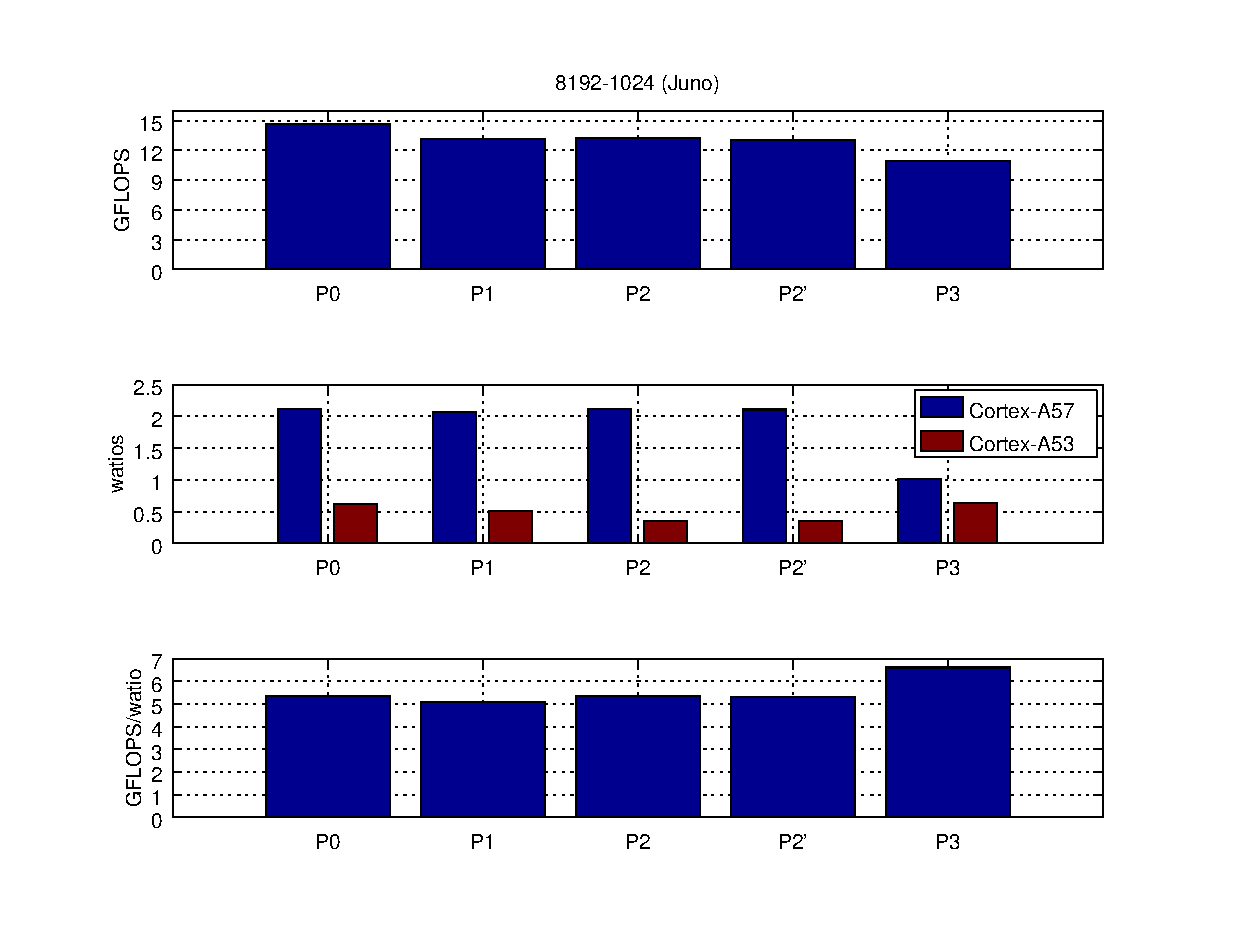
\includegraphics[width=0.9\textwidth]{Plots/dvfs_results/8192-124_0-4_juno.eps}}
      \caption{\juno}
    \end{subfigure}

    \vspace{0.5cm}

    \begin{subfigure}{0.75\textwidth}
      \centering
      \fbox{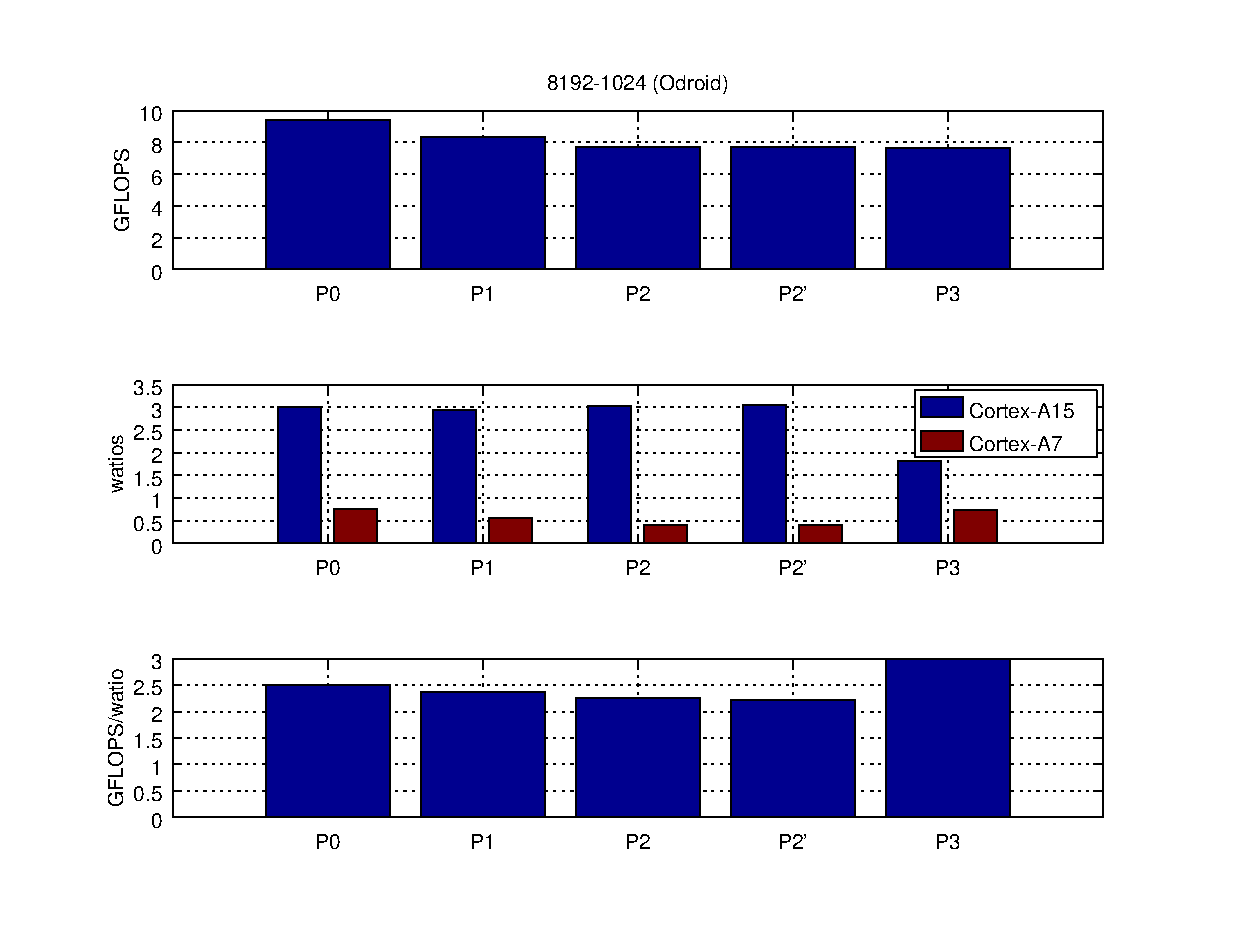
\includegraphics[width=0.9\textwidth]{Plots/dvfs_results/8192-124_0-4_odroid.eps}}
      \caption{\odroid}
    \end{subfigure}  
  \caption{Detalle de las políticas P1-P3 para la configuración
    \texttt{m=8192} y \texttt{b=1024}}
  \label{fig:detalle:p1-p4}
\end{figure}

%%Por último, destacar como una posible conclusión a estos experimentos, cómo
%%el cluster LITTLE refleja que no posee mucho margen de mejora energética,
%%mientras que el cluster big sí. Este hecho se verá respaldado por los
%%resultados de las políticas P4-P6 que se muestran en la siguiente sección.

\subsection{Análisis de resultados para las políticas P4-P6}

\subsubsection{Políticas P4 y P5}

Mientras las políticas anteriores dividían el espacio de frecuencias en
partes iguales respecto al tamaño máximo de la cola, las políticas P4-P6 no
disponen de un punto claro en la ejecución donde desactivar el cluster
correspondiente. Al igual que en las otras políticas, se ha decidido que
este punto esté reflejado por la relación entre el tamaño actual de la cola
de tareas listas frente al tamaño máximo alcanzado hasta el momento. Los
experimentos realizados contemplan desde ejecuciones que desactivan el
cluster cuando el número de tareas listas para ejecución es un $50\%$ del
tamaño máximo alcanzado, decreciendo hasta un punto de corte del $10\%$
respecto al tamaño máximo en intervalos de un $10\%$ del tamaño máximo.
Nótese que este porcentaje no se encuentra relacionado con el tiempo de
ejecución, sino con el número de tareas listas en cada momento. A modo
informativo, la Tabla~\ref{tab:tam-colas-tiempo} muestra para cada
configuración del tamaño de la matriz y bloque (columnas), y para cada
experimento lanzado (filas), el porcentaje del tiempo de ejecución en el
que el cluster se encuentra desactivado para la política P4 y la plataforma
\juno.

\begin{table}
  \centering
  \caption{Porcentaje de tiempo de ejecución en el que el cluster se
    encuentra desactivado en función del momento elegido para desactivar.}
  \label{tab:tam-colas-tiempo}
  {\scriptsize
    \begin{tabular}{cccccccccccccccc}
      \toprule
      \multicolumn{2}{c}{\phantom{a}} & \multicolumn{14}{c}{Tamaño de la matriz \texttt{(m)} y
                                        de bloque \texttt{(b)}.} \\ \cmidrule{2-16}
      \phantom{4} & \texttt{(m)} & \multicolumn{2}{c}{1024} & \multicolumn{2}{c}{2048} &                                                                         \multicolumn{2}{c}{4096} & \multicolumn{2}{c}{4608} & \multicolumn{2}{c}{5120} & \multicolumn{2}{c}{6144} & \multicolumn{2}{c}{8192} \\
      \phantom{a} & \texttt{(b)} & 64 & 128 & 128 & 256 & 256 & 512 & 256 & 512 & 512 & 1024 & 512 & 1024 & 512 & 1024 \\ \hline

{\sc 50\%} & \phantom{a} &69.36 & 45.83 & 39.34 & 55.83 & 43.44 & 50.83 & 39.39 & 38.48 & 40.91 & 42.07 & 39.15 & 35.24 & 40.32 & 48.33 \\
{\sc 40\%} & \phantom{a} &68.20 & 31.25 & 29.29 & 48.75 & 29.41 & 33.33 & 30.61 & 32.73 & 32.73 & 30.54 & 32.83 & 30.42& 30.15 & 37.92 \\
{\sc 30\%} & \phantom{a} &63.42 & 34.58 & 20.89 & 48.33 & 21.14 & 32.50 & 20.88 & 24.85 & 25.00 & 28.06 & 23.08 & 25.43& 21.81 & 33.75 \\
{\sc 20\%} & \phantom{a} &20.40 & 17.92 & 11.64 & 34.17 & 11.40 & 31.67 & 11.97 & 17.27 & 18.41 & 21.04 & 14.56 & 19.12& 13.11 & 26.67 \\
{\sc 10\%} & \phantom{a} &23.10 & 15.00 & 4.90  & 27.92 & 5.27  & 20.00 & 4.87 & 11.52  & 9.55 & 15.13 &7.69 & 10.3 & 5.64 & 12.92 \\ \bottomrule
    \end{tabular}
    \caption*{Política 4 - \juno}
  }

%   {\scriptsize
%     \begin{tabular}{cccccccccccccccc}
%       \toprule
%       \multicolumn{2}{c}{\phantom{a}} & \multicolumn{14}{c}{Tamaño de la matriz \texttt{(m)} y
%                                         de bloque \texttt{(b)}.} \\ \cmidrule{2-16}
%       \phantom{4} & \texttt{(m)} & \multicolumn{2}{c}{1024} & \multicolumn{2}{c}{2048} &                                                                         \multicolumn{2}{c}{4096} & \multicolumn{2}{c}{4608} & \multicolumn{2}{c}{5120} & \multicolumn{2}{c}{6144} & \multicolumn{2}{c}{8192} \\
%       \phantom{a} & \texttt{(b)} & 64 & 128 & 128 & 256 & 256 & 512 & 256 & 512 & 512 & 1024 & 512 & 1024 & 512 & 1024 \\ \hline

% {\sc 50\%} & \phantom{a} &      80.88 & 63.75 & 80.82 & 57.08 & 67.34 & 53.75 & 72.37 & 53.33 & 54.55 & 0.00 & 43.41 & 0.00 & 55.15 & 60.00 \\
% {\sc 40\%} & \phantom{a} &      32.84 & 52.50 & 57.90 & 51.25 & 54.90 & 45.00 & 54.65 & 43.33 & 45.68 & 0.00 & 35.30 & 0.00 & 34.19 & 50.83 \\
% {\sc 30\%} & \phantom{a} &      54.90 & 28.33 & 34.38 & 44.58 & 59.93 & 40.00 & 22.37 & 40.00 & 31.82 & 0.00 & 28.98 & 0.00 & 23.96 & 42.50 \\
% {\sc 20\%} & \phantom{a} &      19.79 & 35.83 & 21.69 & 30.83 & 26.41 & 32.92 & 39.47 & 27.27 & 29.32 & 0.00 & 19.64 & 0.00 & 12.38 & 31.25 \\
% {\sc 10\%} & \phantom{a} &      9.80 & 0.00 & 13.73 & 25.00 & 15.20 & 22.50 & 9.69 & 22.42 & 19.77 & 0.00 & 12.64 & 0.00 & 8.21 & 22.50 \\\bottomrule
%     \end{tabular}
%     \caption*{Política 4 - \odroid}
%   }

\end{table}


La Figura~\ref{fig:p4-p5} muestra el comportamiento de las políticas P4 y
P5 para la plataforma \juno, combinando para cada configuración de tamaño
de matriz y bloque los distintos tamaños de cola experimentados. 
Adicionalmente, se incorporan las medidas realizadas sobre el planificador
\botlev para poder comparar los resultados (columna izquierda en cada
conjunto de datos).

La primera observación que se puede realizar sobre los datos obtenidos es
el impacto muy significativo que posee variar el punto de desactivado del
cluster sobre el rendimiento final de la aplicación, tanto desactivando el
cluster \LITTLE (política P4) como desactivando el cluster \BIG (política
P5). La Tabla~\ref{tab:p4-p5:gflops} muestra el rendimiento alcanzado por
cada configuración del problema, política y plataforma según el momento
elegido para desactivar el cluster correspondiente. Nótese que mientras que
en la plataforma \juno es la política P4 la que obtiene peor rendimiento
frente a la política P5, en la plataforma \odroid sucede al contrario. Una
de las causas que provoca este hecho se encuentra en el tamaño de cada
cluster en cada una de las plataformas. En \juno, el cluster \BIG se
encuentra formado únicamente por dos núcleos, mientras que el cluster
\LITTLE se encuentra formado por cuatro. Al desactivar el cluster \LITTLE,
únicamente se disponen de dos núcleos donde ejecutar las tareas, por lo que
el grado de paralelismo explotado es menor que si se desactiva el cluster
\BIG. Como conclusión adicional, se puede observar cómo, a pesar de que el
rendimiento de un core \BIG (Cortex-A57 en este caso) es más elevado que el
rendimiento de un core \LITTLE (\mbox{Cortex-A53}), realizar la ejecución sobre
cuatro cores \LITTLE obtiene un rendimiento mayor que realizarla sobre
únicamente dos cores \BIG.


\begin{table}
  \centering
  \caption{Rendimiento obtenido para las políticas P4 y P5 en ambas
    plataformas en relación a una ejecución normal con \botlev.}
  \label{tab:p4-p5:gflops}
  {\scriptsize
    \begin{tabular}{rcccccccccccc}
      \toprule
      \phantom{a} & \phantom{a} & \multicolumn{5}{c}{\juno} & \phantom{a} & \multicolumn{5}{c}{\odroid}\\
      \phantom{a} & \phantom{a} & 10\% & 20\% & 30\% & 40\% & 50\% & \phantom{a} & 10\% & 20\% & 30\% & 40\% & 50\% \\\hline

{\sc P4} & \phantom{a} & 52.18\% & 59.56\% & 67.33\% & 78.29\% & 85.87\% & \phantom{a} & 70.477\% & 75.93\% & 82.19\% & 87.55\% & 91.43\%\\
{\sc P5} & \phantom{a} & 58.2\% & 62.99\% & 69.85\% & 76.05\% & 84.77\% & \phantom{a} &61.96\% & 67.85\% & 74.59\% & 82.03\% & 90.27\%\\\bottomrule
    \end{tabular}
  }
\end{table}





\begin{figure}
  \centering
    \begin{subfigure}{0.75\textwidth}
      \centering
      \fbox{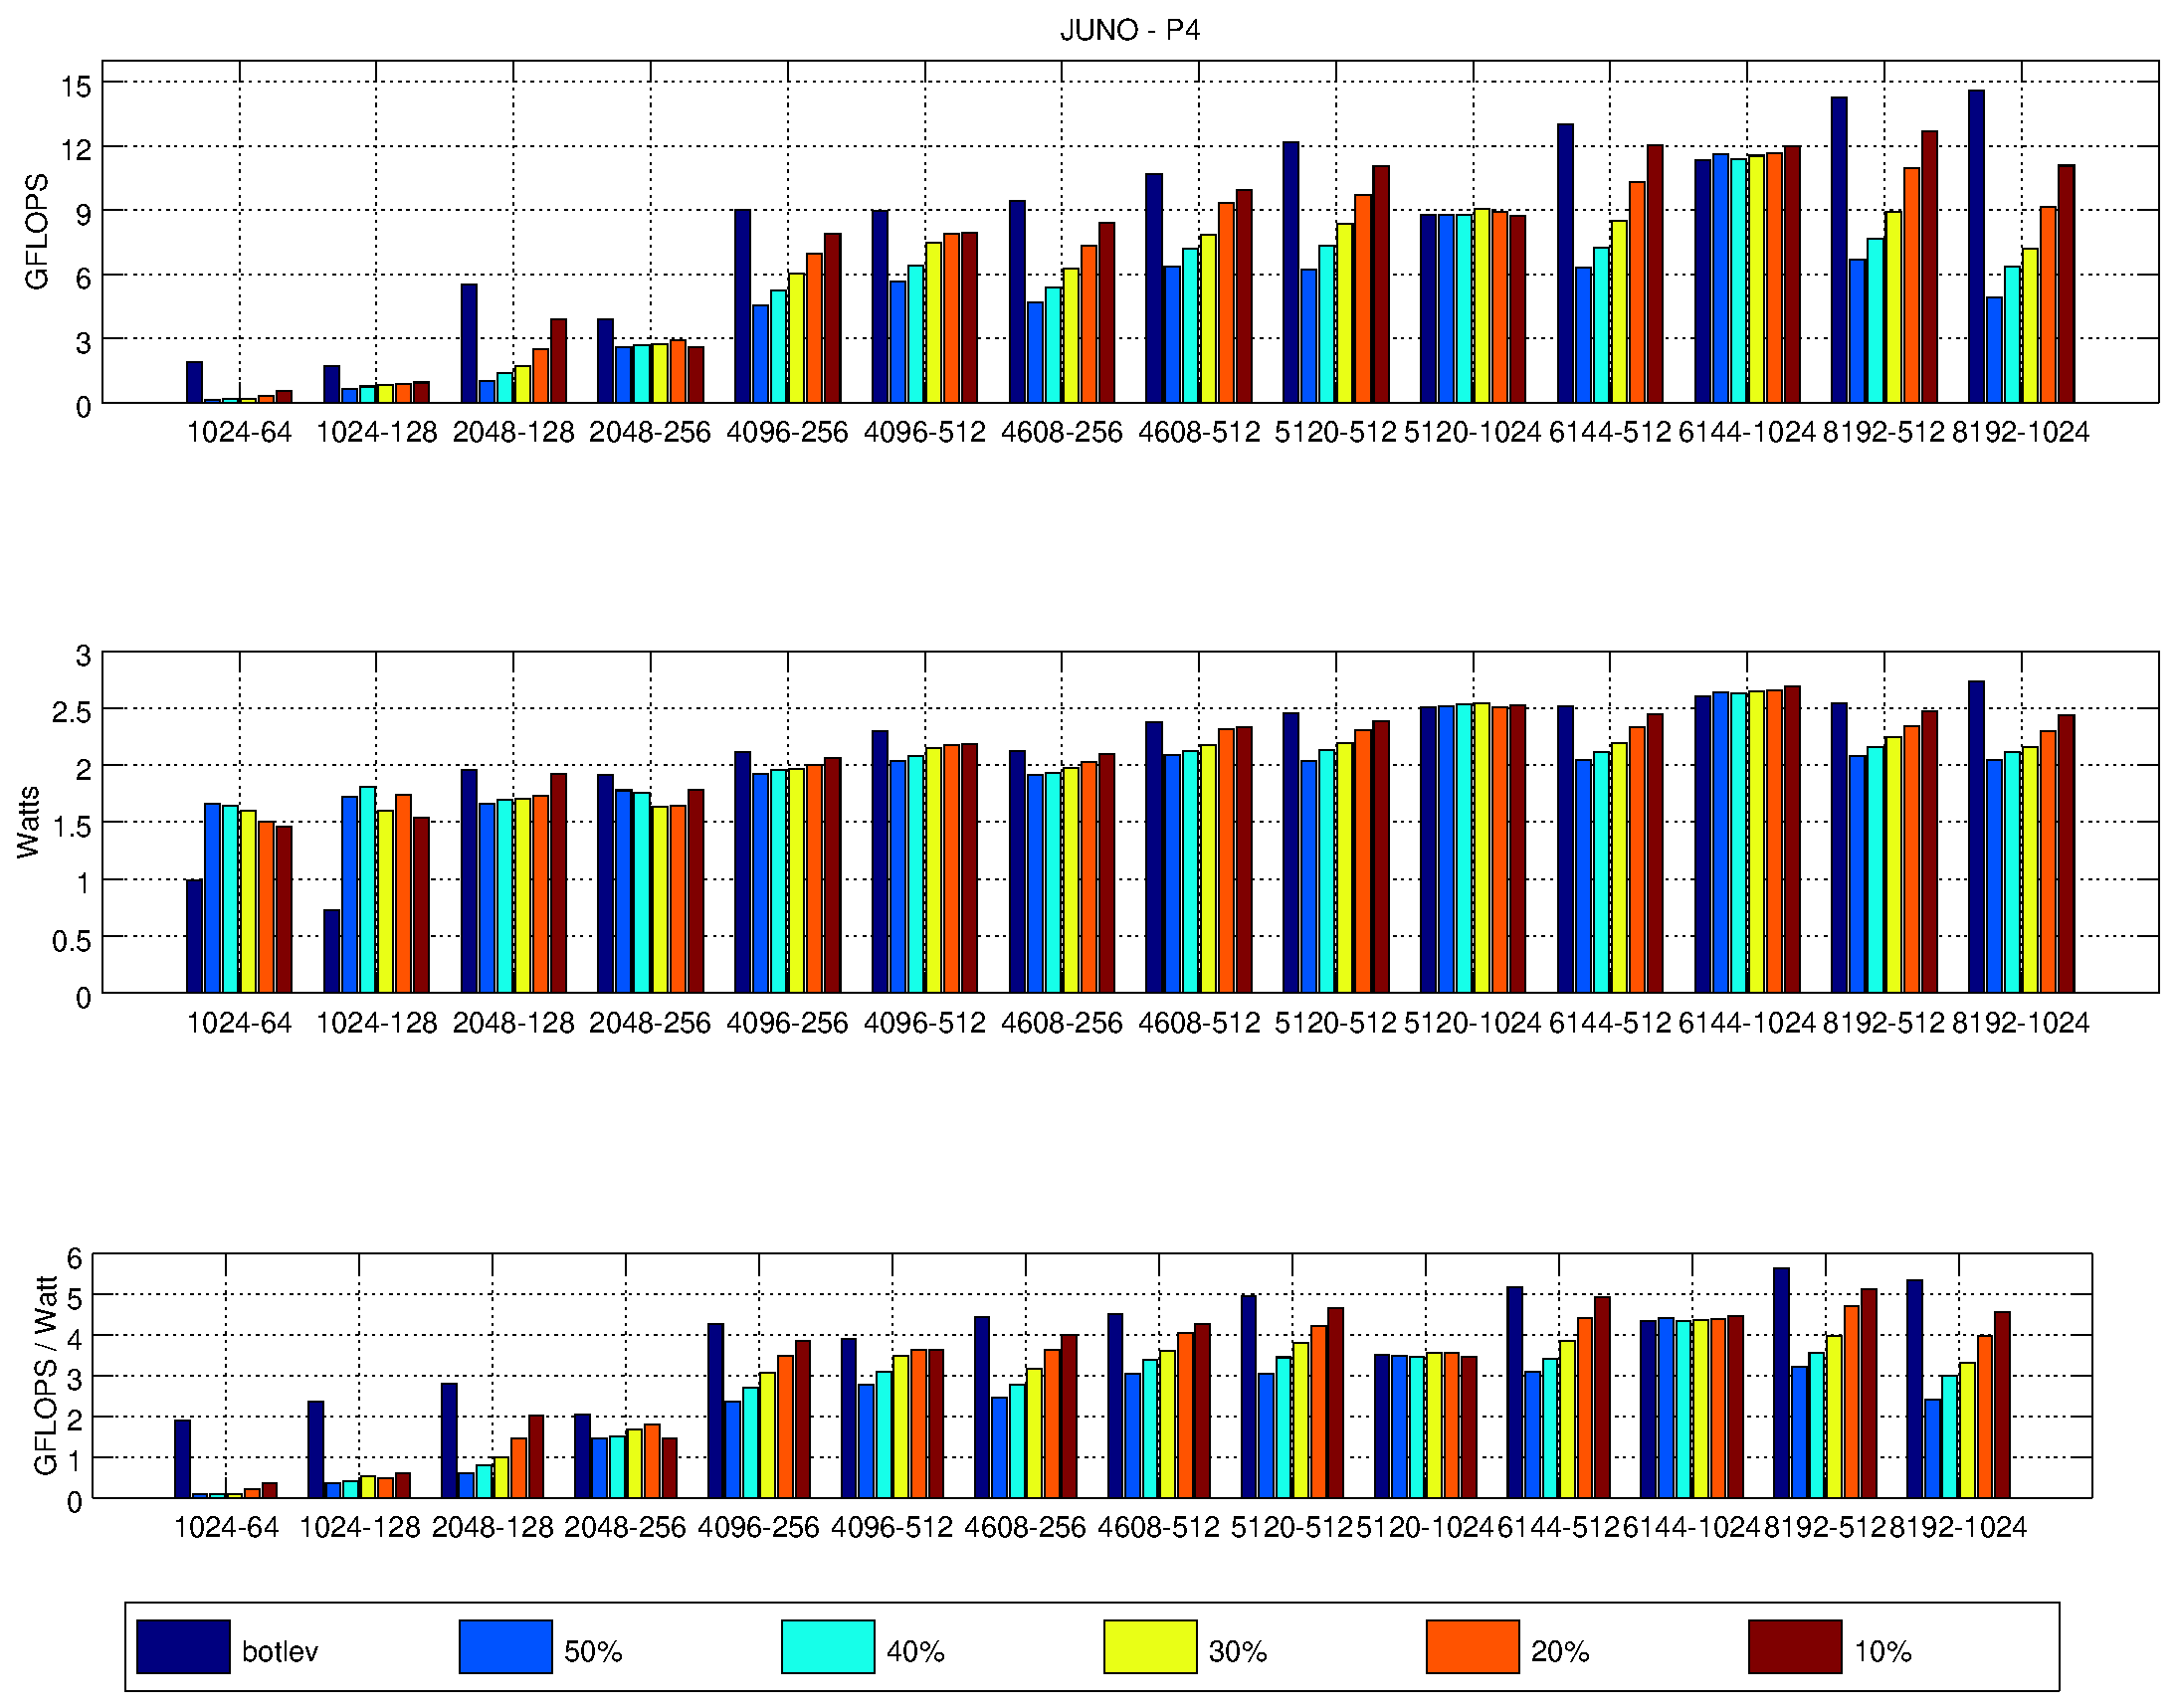
\includegraphics[width=0.9\textwidth]{Plots/sched_results/P4_juno.eps}}
      \caption{P4}
    \end{subfigure}

    \vspace{0.5cm}

    \begin{subfigure}{0.75\textwidth}
      \centering
      \fbox{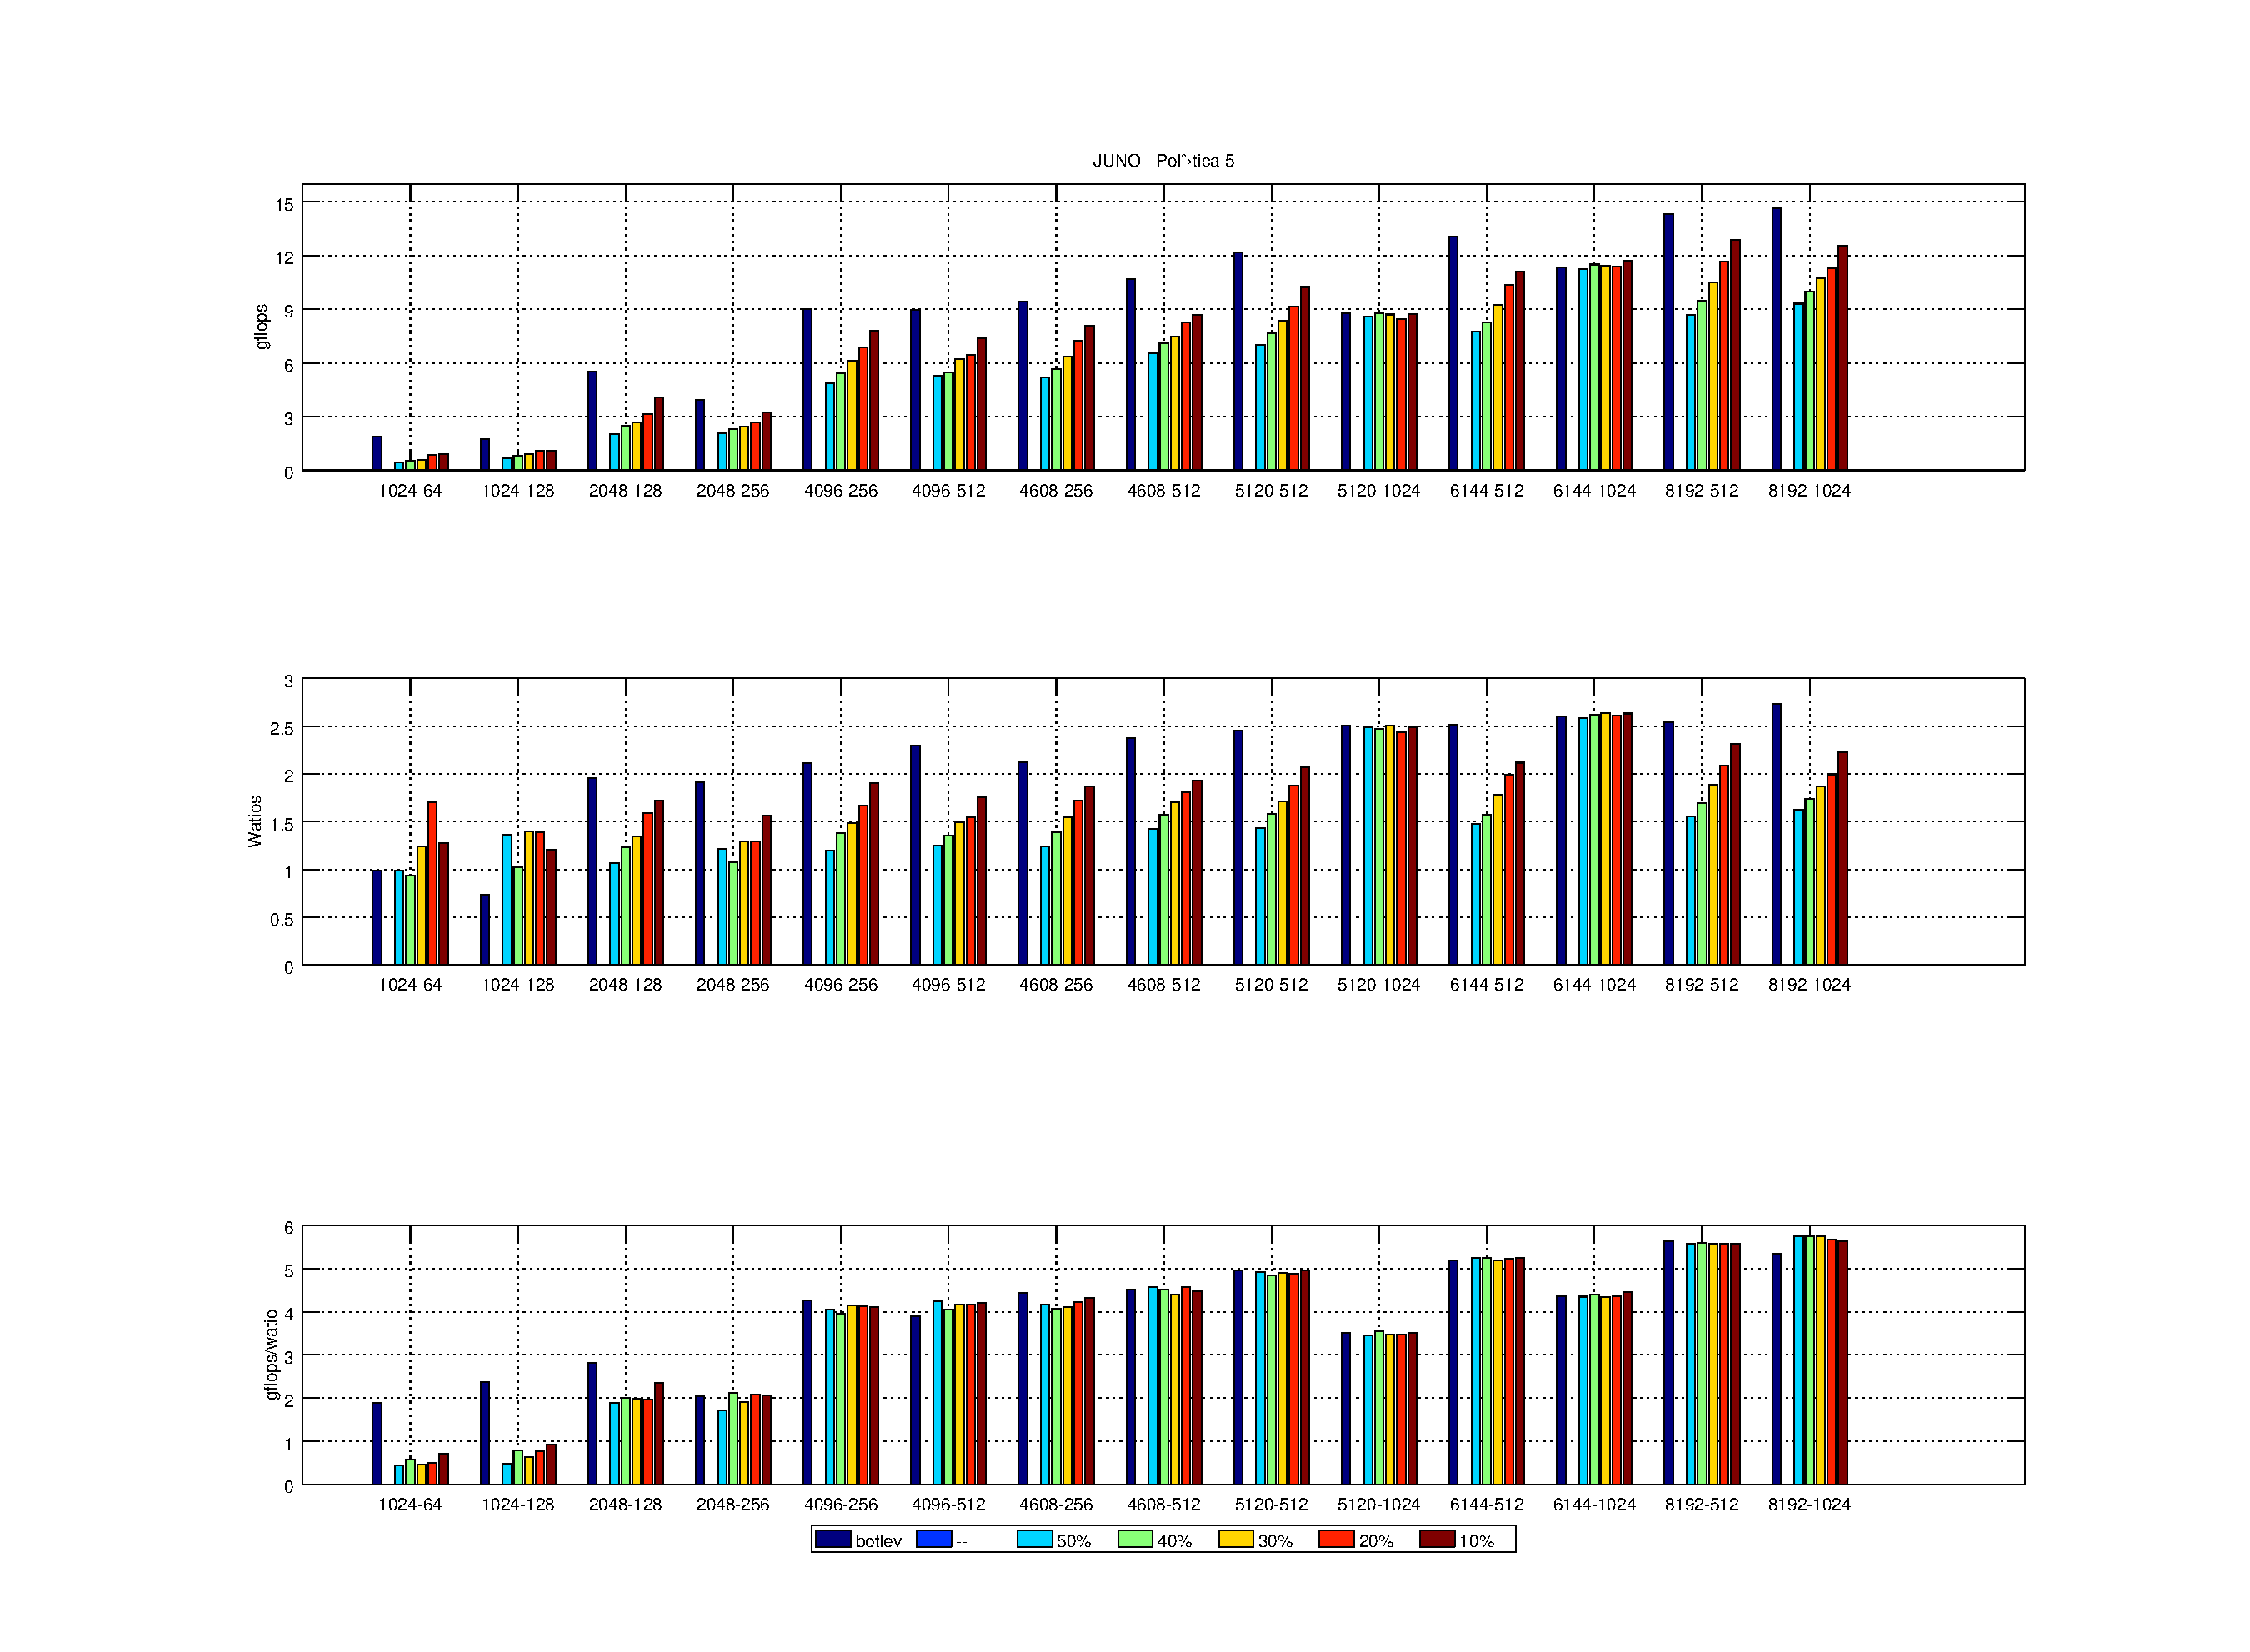
\includegraphics[width=0.9\textwidth]{Plots/sched_results/P5_juno.eps}}
      \caption{P5}
    \end{subfigure}  
  \caption{Resultados para los experimentos P4 y P5 sobre la plataforma
    \juno.}
  \label{fig:p4-p5}
\end{figure}


Como se puede apreciar en la figura, tanto la política P4 como la política
P5 no consiguen obtener la mejora energética buscada. Mientras que la
política P4 obtiene resultados muy inferiores a la ejecución con \botlev,
la política P5 alcanza resultados cercanos. La
Tabla~\ref{tab:mejora-gflopsw-p5} muestra con detalle la diferencia de
rendimiento energético con la ejecución de referencia con \botlev para la
política P5 con cada configuración de tamaño.

A la vista de los resultados, y aunque la política P5 no consiga obtener mejoras
en el rendimiento energético, señalar que consigue resultados similares a
la ejecución convencional reduciendo la potencia instantánea consumida, aunque a
costa de reducir el rendimiento computacional. Sin embargo, esta política
puede tener su utilidad en problemas donde su ejecución esté limitada por
la potencia consumida y no tanto por el rendimiento conseguido, pudiendo
alcanzar un compromiso entre rendimiento y potencia sin afectar al
rendimiento energético final escogiendo el valor adecuado para determinar
cuándo desactivar el cluster.

%%% GFLOPSW %%%%
\begin{table}
  \centering
  \caption[Mejora eficiencia energética para la política P5]{Mejora relativa a la ejecución sobre \botlev de la eficiencia energética para la política P5 en ambas plataformas.}
  \label{tab:mejora-gflopsw-p5}
  {\scriptsize
    \begin{tabular}{cccccccccccccccc}
      \toprule
  \multicolumn{2}{c}{\phantom{a}} & \multicolumn{14}{c}{Tamaño de la matriz \texttt{(m)} y
                                        de bloque \texttt{(b)}.} \\ \cmidrule{2-16}
      \phantom{4} & \texttt{(m)} & \multicolumn{2}{c}{1024} & \multicolumn{2}{c}{2048} &                                                                         \multicolumn{2}{c}{4096} & \multicolumn{2}{c}{4608} & \multicolumn{2}{c}{5120} & \multicolumn{2}{c}{6144} & \multicolumn{2}{c}{8192} \\
      \phantom{a} & \texttt{(b)} & 64 & 128 & 128 & 256 & 256 & 512 & 256 & 512 & 512 & 1024 & 512 & 1024 & 512 & 1024 \\ \hline



{\sc 10\%} & \phantom{a} & \br{-3.666} & \fg{4.066} & \br{-2.797} & \br{-1.841} & \br{-0.523} & \br{-0.270} & \br{-0.515} & \br{-0.370} & \br{-0.324} & \fg{0.045} & \br{-0.328} & \br{-0.076} & \br{-0.440} & \br{-0.222} \\               
{\sc 20\%} & \phantom{a} & \br{-3.978} & \fg{1.981} & \br{-2.589} & \br{-1.773} & \br{-0.303} & \br{-0.162} & \br{-0.478} & \br{-0.234} & \br{-0.247} & \br{-0.001} & \br{-0.269} & \fg{0.002} & \br{-0.283} & \br{-0.133} \\
{\sc 30\%} & \phantom{a} & \br{-4.033} & \br{-0.991} & \br{-2.248} & \br{-1.422} & \br{-0.154} & \br{-0.120} & \br{-0.267} & \br{-0.134} & \br{-0.122} & \fg{0.001} & \br{-0.152} & \br{-0.035} & \br{-0.286} & \br{-0.025} \\ 
{\sc 40\%} & \phantom{a} & \br{-3.693} & \fg{1.560} & \br{-2.451} & \br{-1.077} & \fg{0.055} & \br{-0.057} & \br{-0.154} & \br{-0.008} & \br{-0.022} & \br{-0.017} & \br{-0.057} & \br{-0.014} & \br{-0.193} & \fg{0.001} \\
{\sc 50\%} & \phantom{a} & \br{-4.037} & \br{-1.470} & \br{-1.052} & \br{-0.881} & \fg{0.156} & \fg{0.038} & \fg{0.065} & \fg{0.013} & \fg{0.052} & \br{-0.005} & \fg{0.002} & \br{-0.033} & \br{-0.114} & \fg{0.080}\\\bottomrule
    \end{tabular}
    \caption*{\odroid}
  }
  {\scriptsize
    \begin{tabular}{cccccccccccccccc}
      \toprule
      \multicolumn{2}{c}{\phantom{a}} & \multicolumn{14}{c}{Tamaño de la matriz \texttt{(m)} y
                                        de bloque \texttt{(b)}.} \\ \cmidrule{2-16}
      \phantom{4} & \texttt{(m)} & \multicolumn{2}{c}{1024} & \multicolumn{2}{c}{2048} &                                                                         \multicolumn{2}{c}{4096} & \multicolumn{2}{c}{4608} & \multicolumn{2}{c}{5120} & \multicolumn{2}{c}{6144} & \multicolumn{2}{c}{8192} \\
      \phantom{a} & \texttt{(b)} & 64 & 128 & 128 & 256 & 256 & 512 & 256 & 512 & 512 & 1024 & 512 & 1024 & 512 & 1024 \\ \hline


{\sc 10\%} & \phantom{a} &\br{-1.451} & \br{-1.876} & \br{-0.921} & \br{-0.322} & \br{-0.218} & \fg{0.356} & \br{-0.270} & \fg{0.065} & \br{-0.043} & \br{-0.063} & \fg{0.067} & \br{-0.000} & \br{-0.051} & \fg{0.393} \\
{\sc 20\%} & \phantom{a} &\br{-1.317} & \br{-1.578} & \br{-0.805} & \fg{0.079} & \br{-0.317} & \fg{0.159} & \br{-0.373} & \fg{0.009} & \br{-0.110} & \fg{0.037} & \fg{0.062} & \fg{0.046} & \br{-0.033} & \fg{0.397} \\
{\sc 30\%} & \phantom{a} &\br{-1.428} & \br{-1.727} & \br{-0.818} & \br{-0.143} & \br{-0.130} & \fg{0.269} & \br{-0.329} & \br{-0.104} & \br{-0.064} & \br{-0.039} & \fg{0.005} & \br{-0.015} & \br{-0.055} & \fg{0.393} \\
{\sc 40\%} & \phantom{a} &\br{-1.392} & \br{-1.593} & \br{-0.837} & \fg{0.037} & \br{-0.150} & \fg{0.273} & \br{-0.220} & \fg{0.066} & \br{-0.066} & \br{-0.047} & \fg{0.037} & \fg{0.005} & \br{-0.047} & \fg{0.315} \\
{\sc 50\%} & \phantom{a} &\br{-1.184} & \br{-1.447} & \br{-0.453} & \fg{0.015} & \br{-0.159} & \fg{0.320} & \br{-0.126} & \br{-0.022} & \br{-0.004} & \fg{0.003} & \fg{0.070} & \fg{0.1\
02} & \br{-0.061} & \fg{0.286}\\

\bottomrule
    \end{tabular}
    \caption*{\juno}
  }
\end{table}


\subsubsection{Política P6}
La figura~\ref{fig:detalle:p5-p6} compara los resultados obtenidos mediante
la política P5 y P6. Como se comentaba en la sección~\ref{sec:p6},
desactivar un core a nivel del kernel tiene un coste asociado al tener que
migrar los procesos a un core activo, hecho que se refleja en que el
rendimiento obtenido en los experimentos para la política P6 sea menor al
obtenido para la política P5. Sin embargo, como en la plataforma \odroid
desactivar el cluster \BIG supone un consumo cercano a cero, las medidas
para la potencia instantánea son muy inferiores a las obtenidas provocando
que los cores estuvieran \emph{idle} pero sin llegar a
desactivarlos. Combinando estos dos resultados se obtiene el rendimiento
energético mostrado en la tabla~\ref{tab:mejora-gflops-p6}. Como se puede
apreciar, la mejora en el consumo de potencia es superior a la pérdida de
rendimiento, consiguiendo ganancias en el rendimiento energético, haciendo
a esta política una solución válida para obtener una mejora de rendimiento
energético consiguiendo reducciones considerables de la potencia disipada
durante la ejecución.

\begin{figure}
  \centering

  \begin{subfigure}{0.9\textwidth}
    \centering
    \fbox{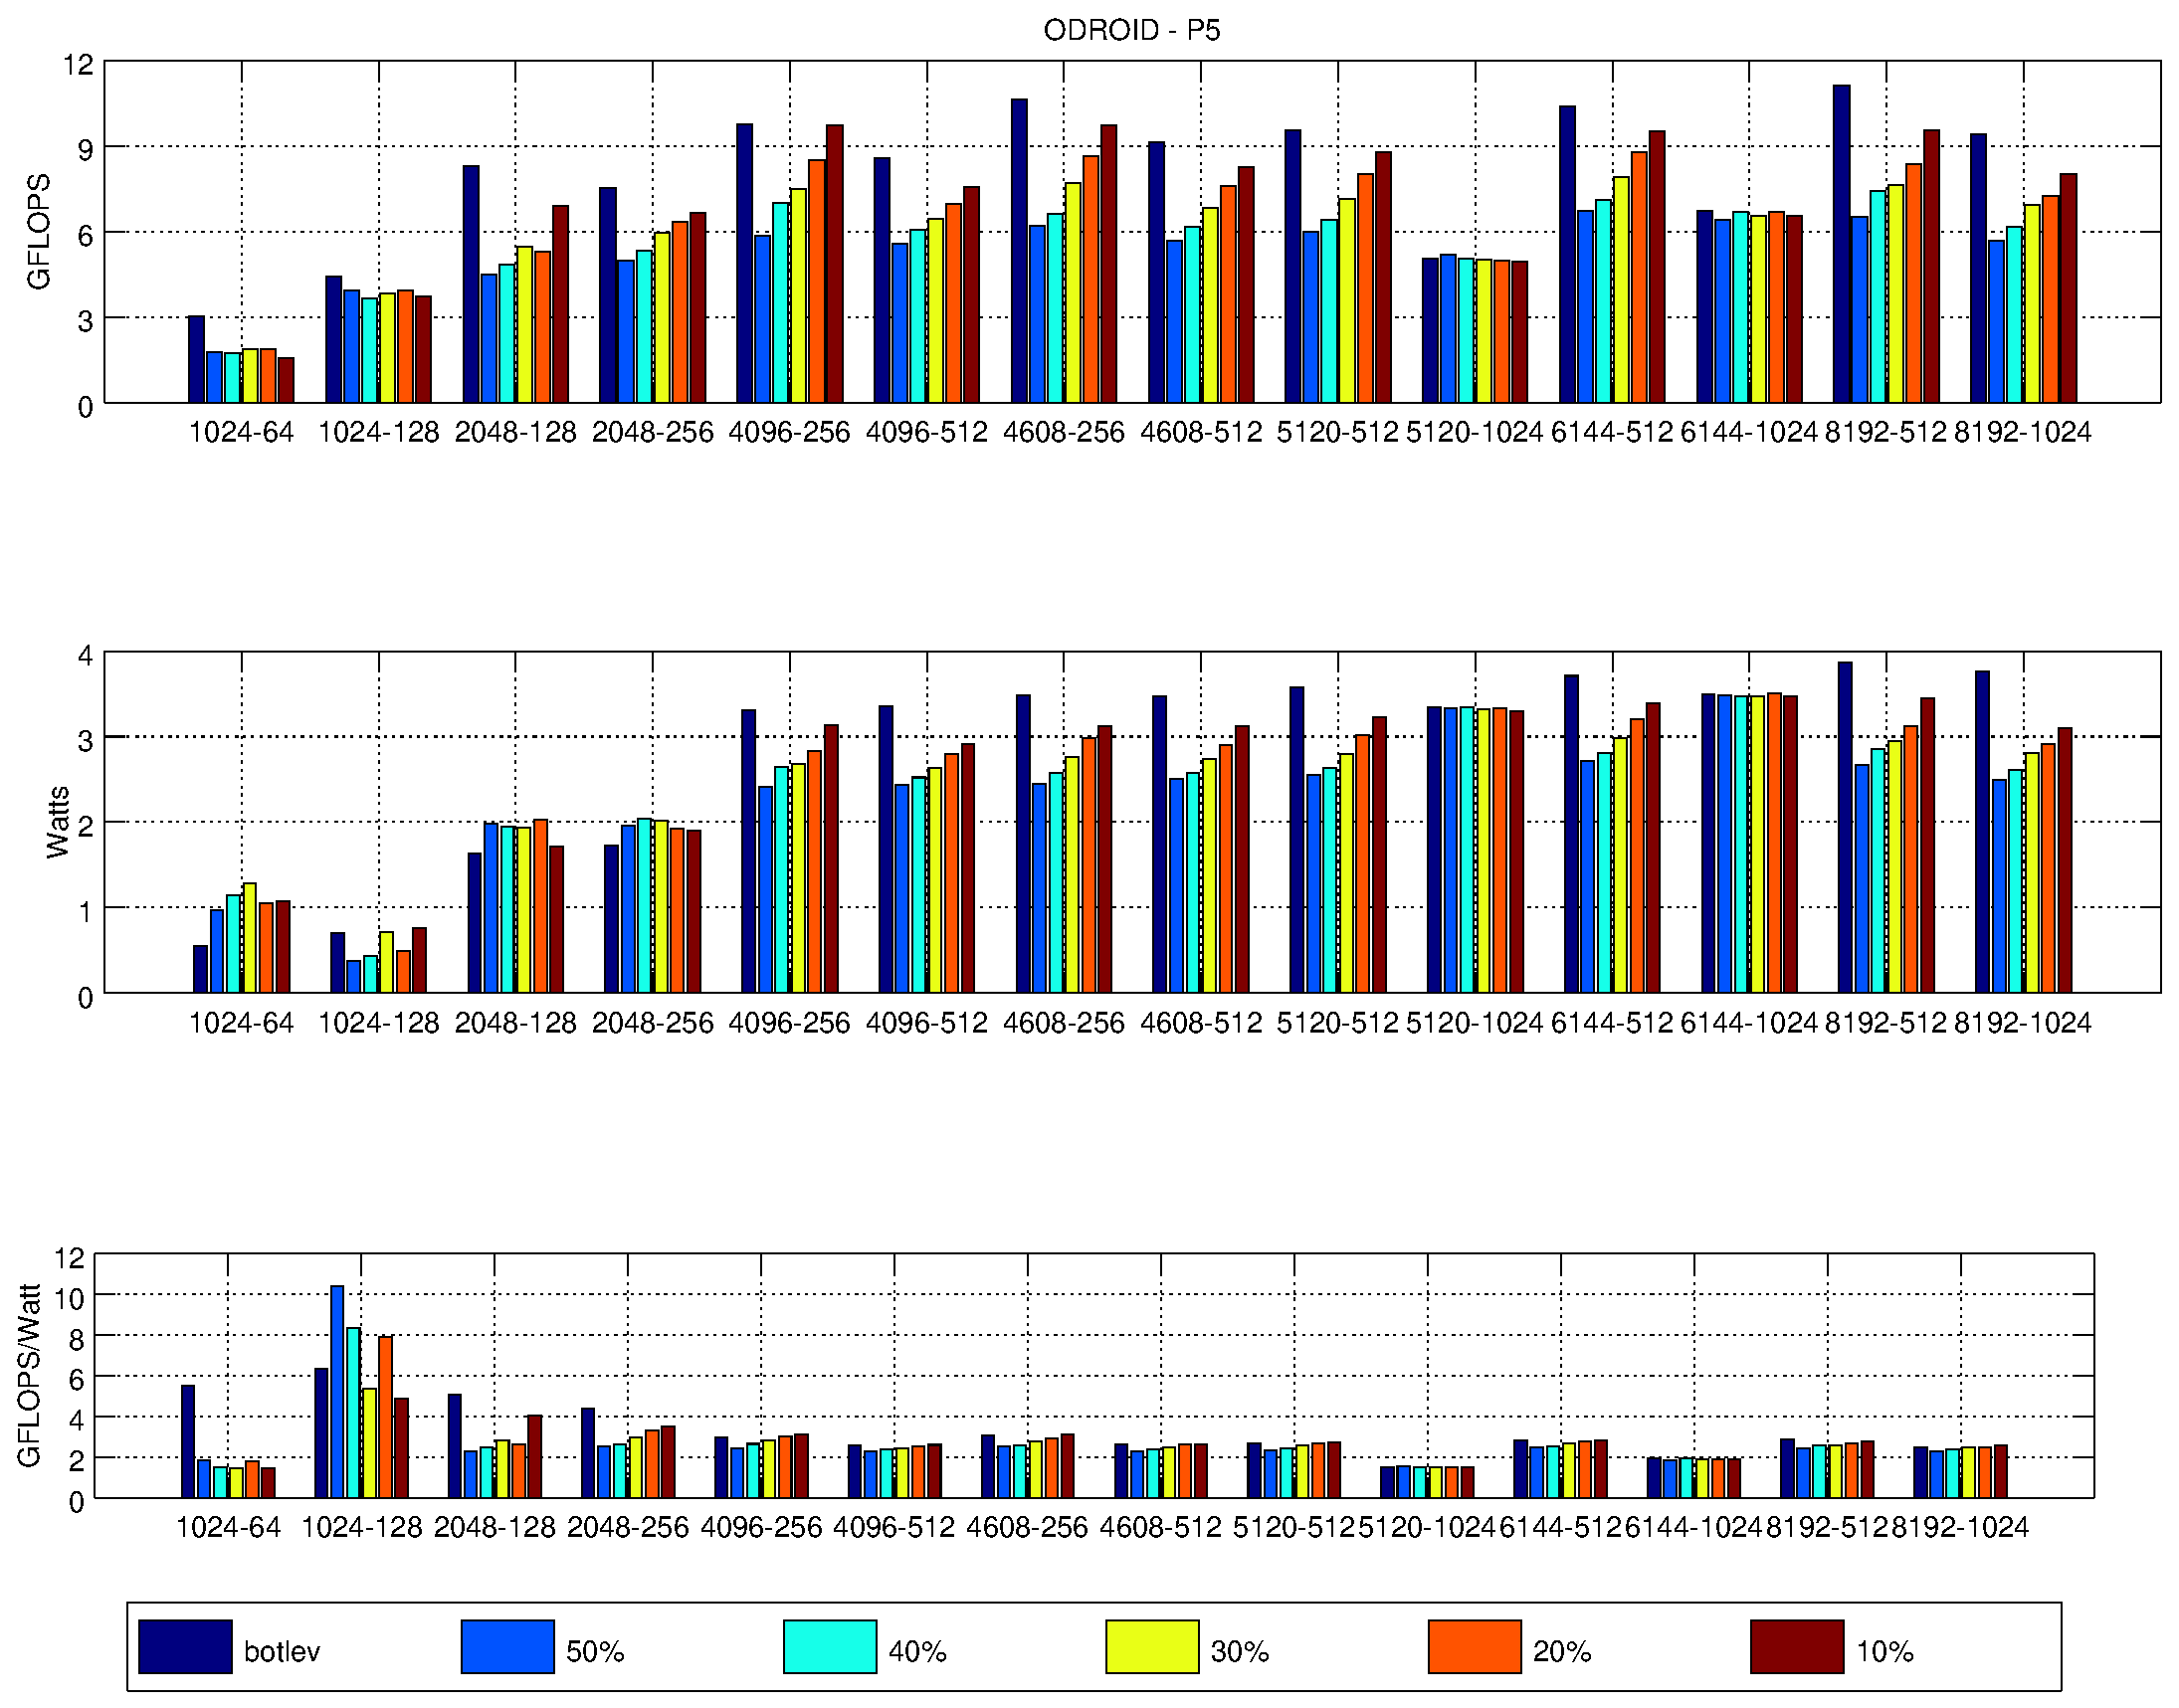
\includegraphics[width=0.9\textwidth]{Plots/sched_results/P5_odroid.eps}}
    \caption*{Política P5}
  \end{subfigure}
  
  \begin{subfigure}{0.9\textwidth}
    \centering
    \fbox{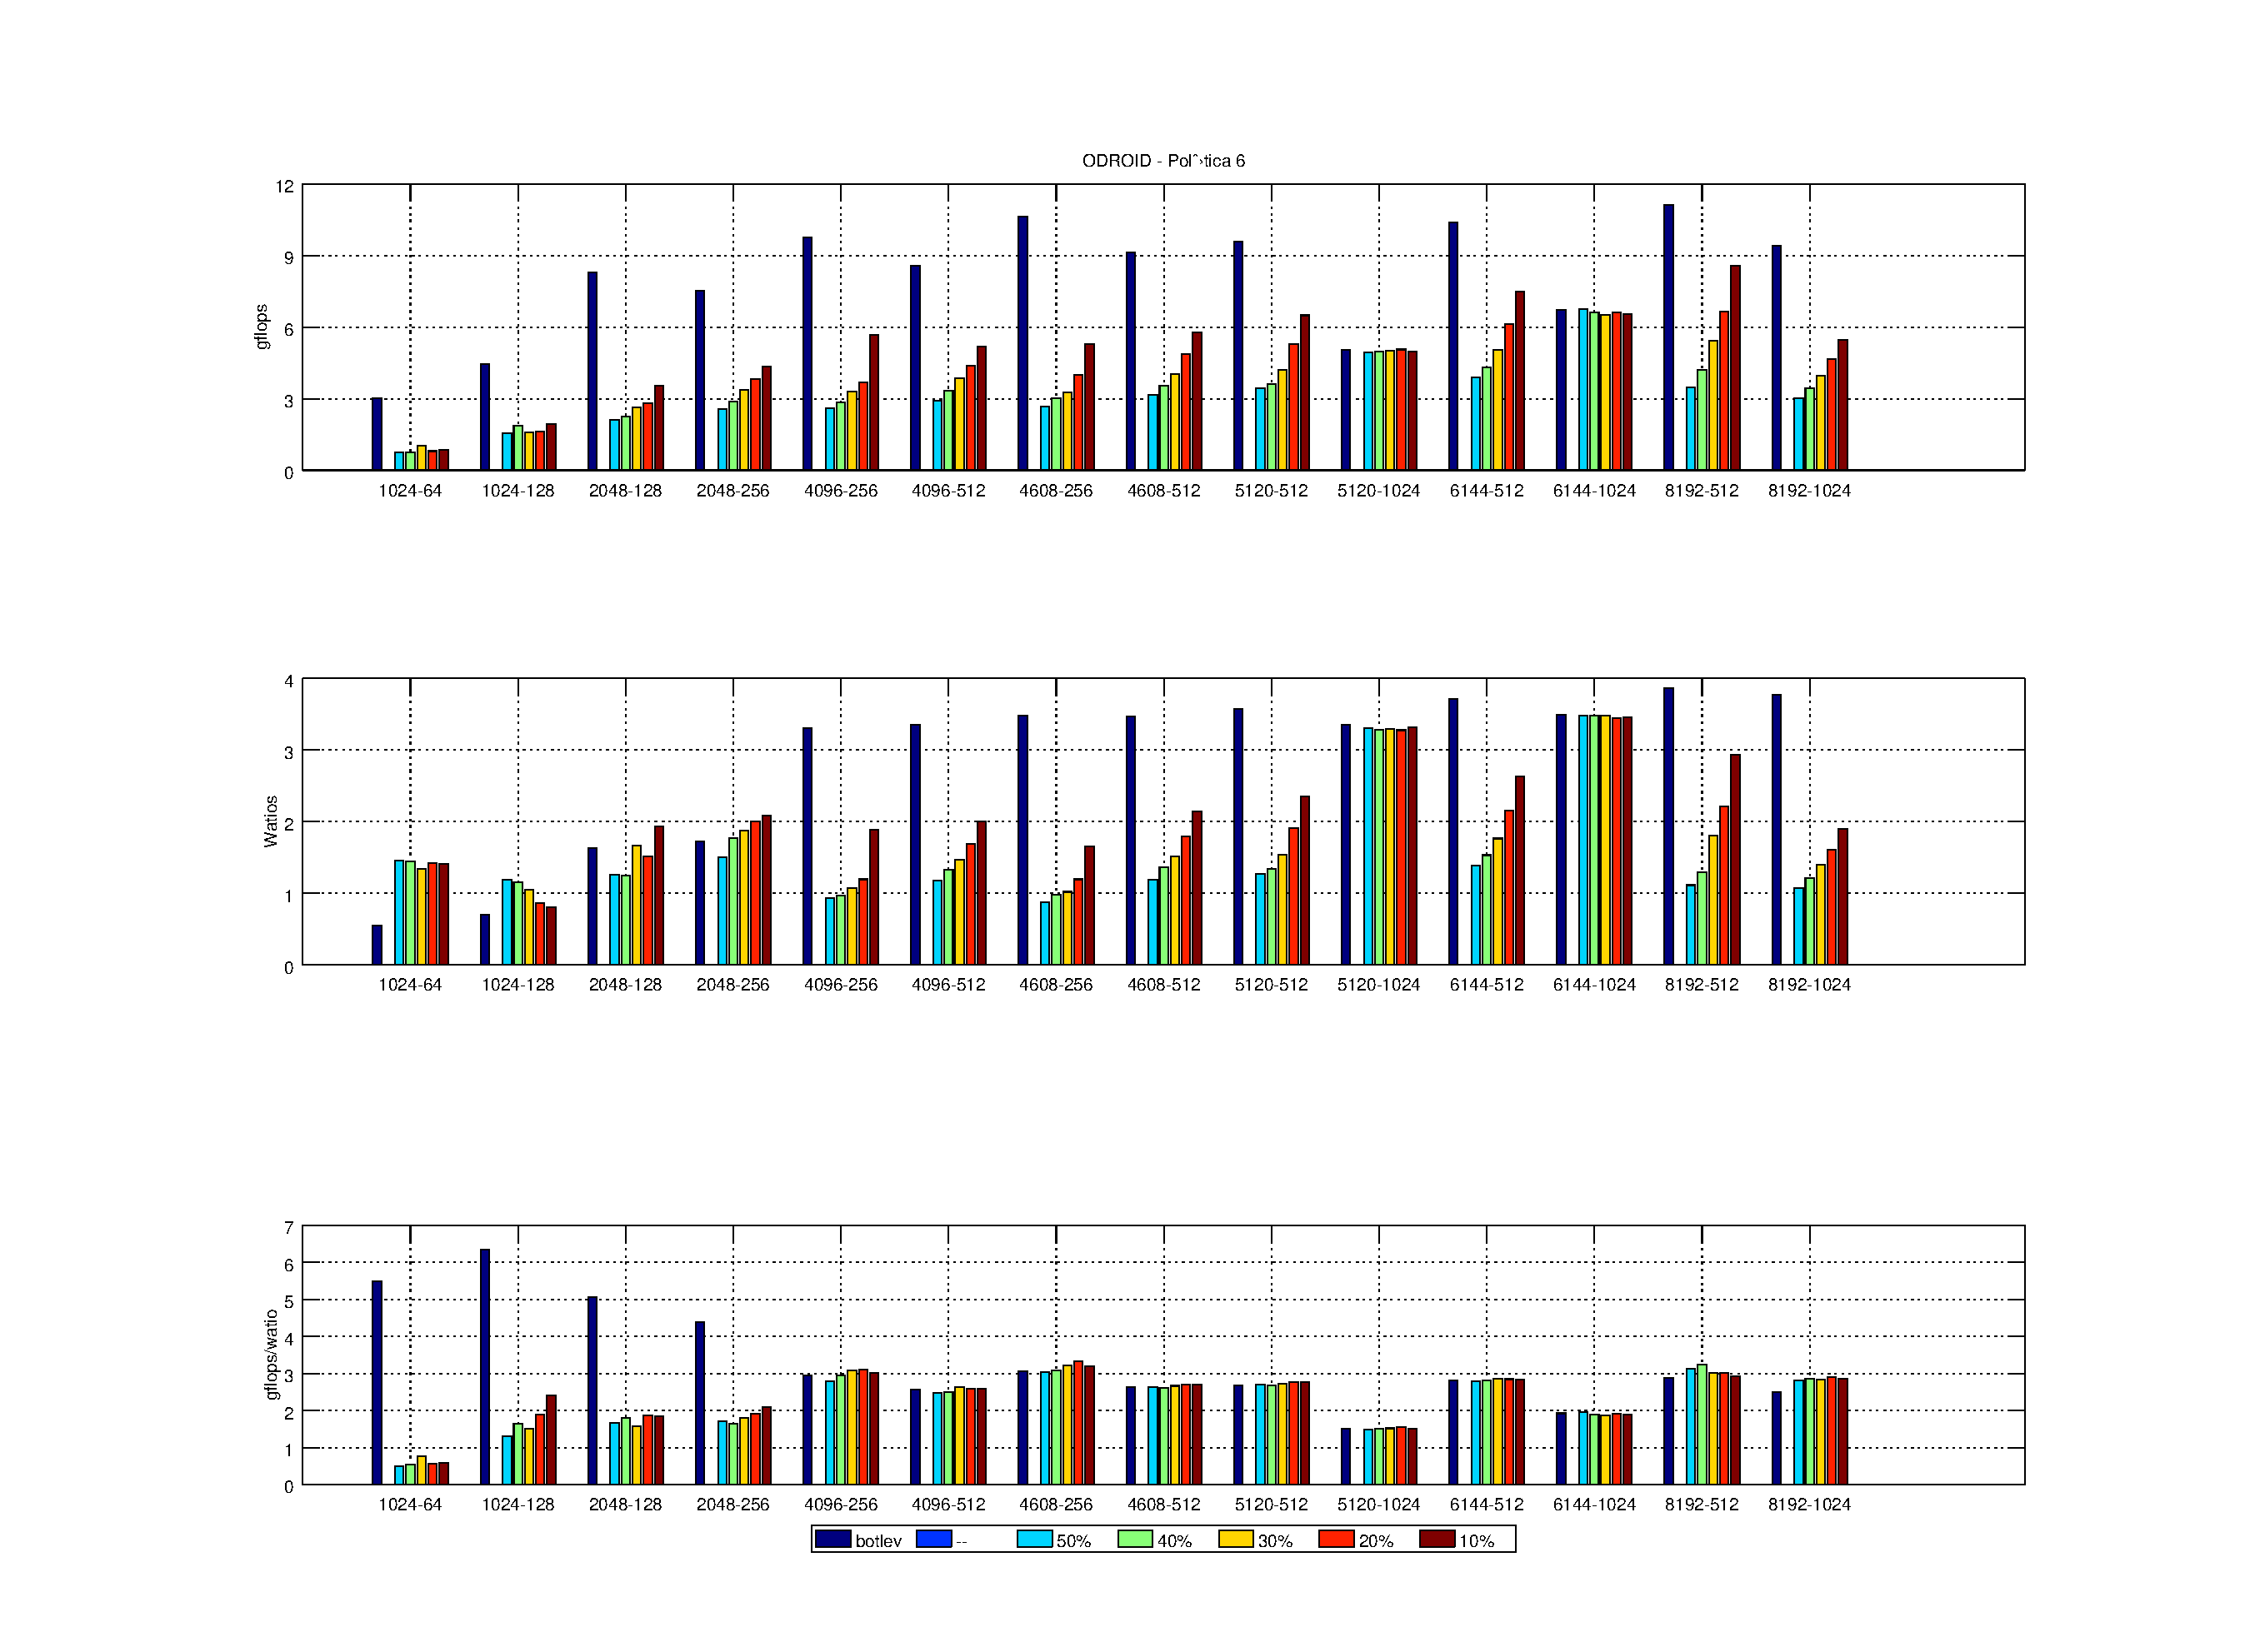
\includegraphics[width=0.9\textwidth]{Plots/sched_results/P6_odroid.eps}}
    \caption*{Política P6}
  \end{subfigure}

  \caption{Resultados de los experimentos realizados para las políticas P5
    y P6 sobre \odroid.}
  \label{fig:detalle:p5-p6}
\end{figure}



\begin{table}
  \centering
  \caption[Mejora eficiencia energética para la política P6]{Mejora de la
    eficiencia energética para la política P6.}
  \label{tab:mejora-gflopsw-p6}
  {\scriptsize
    \begin{tabular}{cccccccccccccccc}
      \toprule
  \multicolumn{2}{c}{\phantom{a}} & \multicolumn{14}{c}{Tamaño de la matriz \texttt{(m)} y
                                        de bloque \texttt{(b)}.} \\ \cmidrule{2-16}
      \phantom{4} & \texttt{(m)} & \multicolumn{2}{c}{1024} & \multicolumn{2}{c}{2048} &                                                                         \multicolumn{2}{c}{4096} & \multicolumn{2}{c}{4608} & \multicolumn{2}{c}{5120} & \multicolumn{2}{c}{6144} & \multicolumn{2}{c}{8192} \\
      \phantom{a} & \texttt{(b)} & 64 & 128 & 128 & 256 & 256 & 512 & 256 & 512 & 512 & 1024 & 512 & 1024 & 512 & 1024 \\ \hline


{\sc 10\%} & \phantom{a} &\br{-4.984} & \br{-5.028} & \br{-3.400} & \br{-2.671} & \br{-0.160} & \br{-0.085} & \br{-0.021} & \fg{0.009} & \fg{0.015} & \br{-0.019} & \br{-0.008} & \fg{0.023} & \fg{0.239} & \fg{0.325}\\
{\sc 20\%} & \phantom{a} &\br{-4.956} & \br{-4.707} & \br{-3.278} & \br{-2.745} & \fg{0.004} & \br{-0.053} & \fg{0.034} & \br{-0.031} & \fg{0.008} & \fg{0.006} & \fg{0.008} & \br{-0.024} & \fg{0.350} & \fg{0.350} \\
{\sc 30\%} & \phantom{a} &\br{-4.718} & \br{-4.830} & \br{-3.490} & \br{-2.578} & \fg{0.124} & \fg{0.070} & \fg{0.162} & \fg{0.036} & \fg{0.047} & \fg{0.009} & \fg{0.052} & \br{-0.047} & \fg{0.127} & \fg{0.347} \\
{\sc 40\%} & \phantom{a} &\br{-4.922} & \br{-4.442} & \br{-3.210} & \br{-2.465} & \fg{0.146} & \fg{0.023} & \fg{0.285} & \fg{0.071} & \fg{0.086} & \fg{0.034} & \fg{0.043} & \br{-0.006} & \fg{0.124} & \fg{0.408} \\
{\sc 50\%} & \phantom{a} &\br{-4.893} & \br{-3.923} & \br{-3.233} & \br{-2.291} & \fg{0.060} & \fg{0.018} & \fg{0.144} & \fg{0.060} & \fg{0.085} & \br{-0.012} & \fg{0.039} & \br{-0.035} & \fg{0.051} & \fg{0.367} \\

\bottomrule
    \end{tabular}
  }

\end{table}

%-- Configuraciones para emacs --
%%% Local Variables:
%%% mode: latex
%%% TeX-master: "./principal.tex"
%%% End:
